\chapter{Theory}

In this chapter some of the different theories about the moon will be presented. This includes some of the general theories moon about the environment and its characteristics. The theory and some simple calculations about the ice structure and temperature will then be discussed. The definition of life itself will be evaluated and finally the needed descent profile of the lander will be introduced.

\section{Moon Characteristics} % JP, Yannis

% General info: https://en.wikipedia.org/wiki/Colonization_of_Europa

\iffalse
* Rock core, water, ice

    * Why do we think so?
    
    * Geysers?
\fi 

\subsection{Radiation Environment} \label{chap:radiation}%  "landing site guys", "orbiter guys"

%* Both for the orbiter and the lander

Radiation: http://zimmer.csufresno.edu/~fringwal/w08a.jup.txt

\autsubsection{Tidal Wave}{Kristian Sloth Lauszus and Lukas Christensen}

\section{Ice characteristics}
In this section the different theories about the ice characteristics will be presented. This includes the structural profile and a simplified calculation of the ice temperature profile. Furthermore the concept of water convection will be presented, as it might eliminate the needs for low-pressure pump system to circulate the water into the different instruments.

\autsubsection{Structural Profile}{Rasmus Lundby Pedersen}\label{sec:structural_profile}

The first space probe flybys took place in the early 1970s, and Europa quickly became one of the main focuses in the search for past or present extraterrestrial life-harbouring environments, within reachable distances. Already in the 1960's were it discovered from earth-based observations, that the surface of Europa was covered in solid ice, not much unlike other satellites located that deep in the cold reaches of our solar-system. However, data recovered from satellite flybys supplied us with new information about the geology and composition of the moon's surface, having since helped us understanding the of Jupiter's, arguably, most interesting moons with respect to life-supporting environments.\\
\\
The Voayger mission from the late 1970's sent back coarse imagery of Europa with resolution in the ranges of kilometres per pixel, carrying valuable information about the surface of the Jovian satellite\cite{VoyagImg}. More specifically, the images showed a surface resembling that of a ball of string, discarding theories of Europa having a smooth surface, with it in stead being full of bands and ridges.\\%See requested article from DTU Findit
The Galileo spacecraft was launched in 1989 and entered orbit around Jupiter in 1995. It started transmitting data back to earth, from its extensive remote-sensing instrument suite
\iffalse 
(seen on fig. \ref{fig:GalInst1} and \ref{fig:GalInst2})
\fi
 with resolution surpassing Voayger's images almost three orders of magnitude. 
\iffalse
\begin{figure}[htb]
	\centering
	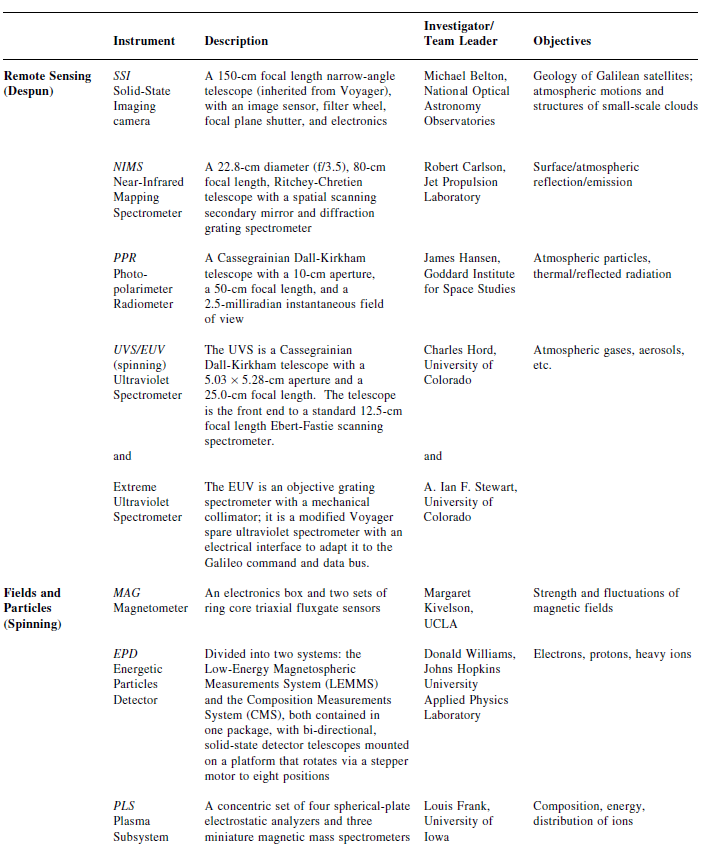
\includegraphics[width=\textwidth]{figures/Rasmus/GalileoInstrument1}
	\caption{Instrument suite of the 1989 Galileo mission.\cite{SciStrat} (\textit{Continued in fig. \ref{fig:GalInst2}}). \label{fig:GalInst1}}
\end{figure}
\begin{figure}[htb]
	\centering
	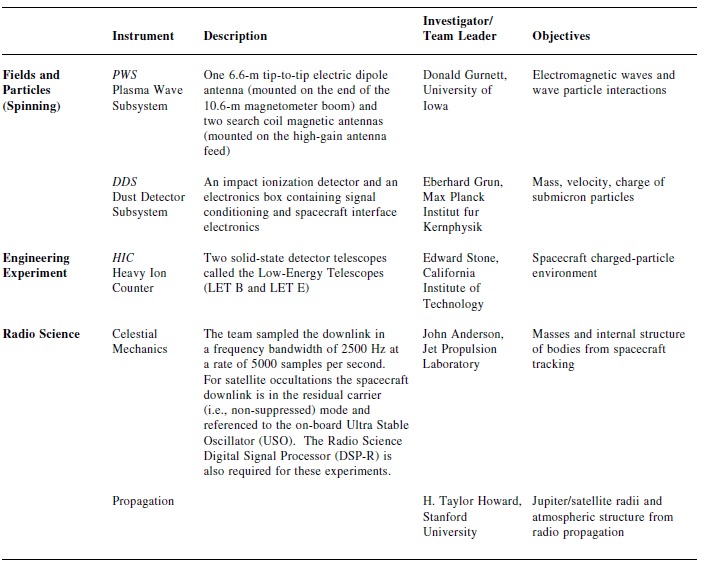
\includegraphics[width=\textwidth]{figures/Rasmus/GalileoInstrument2}
	\caption{Instrument suite of the 1989 Galileo mission.(Continued from fig. \ref{fig:GalInst1}) \cite{SciStrat} .\label{fig:GalInst2}}
\end{figure}
\fi
\\
The high-resolution measurements showed what seemed to be blocks of ice filled with ridges and/or early cracks, that had been lifted and rotated at some point in time. These disruptions indicates that there might be a liquid or softer slushy layer underneath the solid ice surface that through movement had broken and relocated the ice-crust. These cracks are illustrated on fig. \ref{fig:SurfCrack}, which is one picture of a series from the 1989 Galileo satellite\cite{HidOcean}. In any case, it indicates that there is some kind of structural activity in the outermost layer of the moon.\\
\\

\begin{figure}[htb]
	\centering
	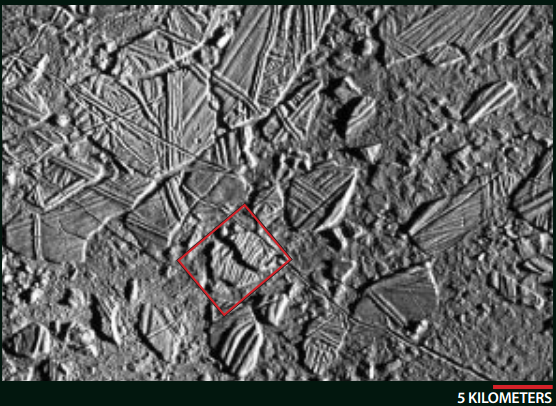
\includegraphics[width=\textwidth]{figures/Rasmus/SurfCrack}
	\caption{Image of Europa's surface taken by the Galileo satellite, showing ridges and disruptions in the surface. \label{fig:SurfCrack}\cite{HidOcean}}
\end{figure}

% Surface Composition
As explained in the study made by the Space Studies Board's Committee on Planetary and Lunar Exploration (COMPLEX), the data from Galileo’s Near-Infrared Mapping Spectrometer (NIMS) show that the water-ice absorption of Europa doesn't match with the expected outcome of pure-water ice, even for areas where the level of frozen sulfur oxide is thought to be lowest (The source of this $SO_2$ is presumably volcanic eruption on Io.). There has been some theories on the cause of this, including the presence of salts and other minerals in the ice but recent studies show that bubbles and fractions could result in the same discrepancies and band shifts in the measurements. However, it is still believed that some of the darker spots seen on the moon are observed because of salts and minerals like hexahedrite, epsomite, and natron\cite{SciStrat}. % INDSÆT The identity of that contaminant so far eludes scientists, but sulfur or iron compounds are suspected from Hidden Ocean P. 8
\\
\\
The actual thickness of the theorized ice-crust, and even the complete structural model of the moon, is still subject to many discussions. It was previously (prior to the Galileo mission) believed that the moon could be consisting of a hydrated silicate core coated in a thin layer of water-ice. However, with the measurements of Europa's gravitational field done by the Galileo satellite has this theory since been largely debunked. The current popular belief is that the cores is either a solid or fluid metallic core surrounded by a layer of water and ice of more than 100km due to the estimated density of the Jovian body. \\
The global ratio between liquid and solid water-ice is still unknown since it must be based on assumptions about the internal structure of the ice, which in themselves are extremely uncertain. The estimates we do have are even based on local imagery, since making them on a global basis requires dedicated orbiter mission, like the planned CLIPPER mission.\\%INDSÆT REFERENCE
In one study, the impact craters of Europa are analysed and compared with computer simulations to estimate regional crust thickness. The rationale is, that central peaks found in craters on the surface resemble material uplift caused by meteor impacts on extraterrestrial planets\cite{ThickImpact}, as seen on fig. \ref{fig:ImpactPic}. Therefore, it is assumed that the crust is thick enough to prevent complete surface penetration from meteor impact and as such they conclude that the ice at the impact sites must have been more than 	$\mathbf{3-4km}$ thick. Graphical representation of the simulation results can be seen on fig. \ref{fig:ImpactSim}. Another study that also investigated the impact craters, and taken from their introduction: "Stereo topographic profiles suggest that the plateau [a plateau SW of Cilix impact crater] is
flexurally supported, with an effective elastic thickness $t_e$ of
$~6km$. For a conductive temperature profile this $t_e$ value
implies a solid ice shell thickness of $\mathbf{~15km}$; if the shell is
convecting, this estimate is a lower bound. Combined with
independent estimates, we infer a probable shell thickness
of $\mathbf{25 km}$. The shell thickness is likely to be uniform over
the entire satellite."\cite{ThermElast}
\begin{figure}[htb]
	\centering
	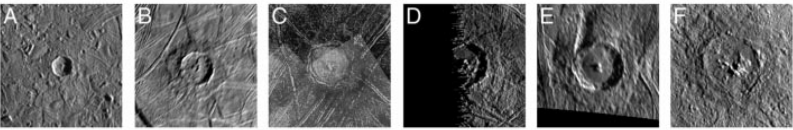
\includegraphics[width=\textwidth]{figures/Rasmus/Impacts}
	\caption{Galileo images of Europan central peak craters. (\textbf{A}) Brigid ($11^\circ$N, $80^\circ$W), $D=8.5km$. (\textbf{B}) Grainne ($60^\circ$S, $95^\circ$W), $D=13.5$km. (\textbf{C}) Cilix ($2.6^\circ$N, $182^\circ$W ), $D18.4$km. (\textbf{D}) Amergin ($14^\circ$S, $230^\circ$W), $D=18.6$km. (\textbf{E}) Maeve ($58^\circ$N, $75^\circ$W ), $D=20.4$km. (\textbf{F}) Pwyll ($25^\circ$S, $271^\circ$W), $D=23.7$ km. All images are at a resolution of 250 m/pixel and each is illuminated from the right except Cilix (\textbf{C}), which was observed at high sun
	\cite{ThickImpact}. D is crater diameter. \label{fig:ImpactPic}}
\end{figure}
\begin{figure}[htb]
	\centering
	\includegraphics[width=1\textwidth]{figures/Rasmus/Impacts2}
	\caption{Model results for impacts of large (A through C) and small projectiles (D through F) into 9-km-thick ice (gray) over liquid water (A) and (D), 5-kmthick ice (gray) over liquid water (black) (B) and (E), and 3-kmthick conductive lid (light gray) over convecting ice (dark gray) (C) and (F). Solid, dotted, and dashed lines show the regions of complete vaporization, complete melting, and $50\%$ melting, respectively.
	\cite{ThickImpact}.\label{fig:ImpactSim}}
\end{figure}
\\
Thermal models has also been used to estimate the average ice shell thickness of Europa. One study is carried out with the assumption of a ice shell decoupled from a silicate core by a layer of liquid water \cite{ThermThick}, so its conclusion may not fit with modern theories. They estimate the shell to have a thickness of $\mathbf{13-25km}$, depending on which thermal rheology model is used (Maxwell and general flow rheology, with and without heat flow from the core). Another thermal model is based on the suggestios of Europa having a metallic core and a silicate mantle, covered by significant layer of liquid water and a thinner ice shell \cite{ThermThick2}. The study heavily relies on convection in the ice, and this complicates the study further. The heat flow through the ice is dependant on the shell thickness, and shell thickness is in turn dependant on the heat flow. This study concludes on the result that the average thickness of a completely frozen shell must be around $\mathbf{36km}$ based on the study's assumptions.
\\
\\ One study carried out by [J.M. Wahr, M.T. Zuber et al., 2006] analyses the tidal effects caused by the differentiating gravitational pull from Jupiter, as Europa travels in its elliptical orbit around the planet. The result of the study is a set of analytical equations estimating the global thickness based on the Love-number of Europa. However, in order to utilize these equations, accurate knowledge of the ice-composition is required, as well as precise estimates of the Love numbers. In the end they even conclude conclude that their results may not be sufficient since they only provide an accuracy of $\pm 5\mathrm{km}$.\\
\\
Apart from the thickness and elemental composition of the ice, internal structure in the shelf is also highly relevant to the planned penetrator mission. Assuming a completely homogeneous ice-shelf is a crude over-simplification and may be a mission-killer if alternatives aren't considered. 
\begin{figure}[htb]
	\centering
	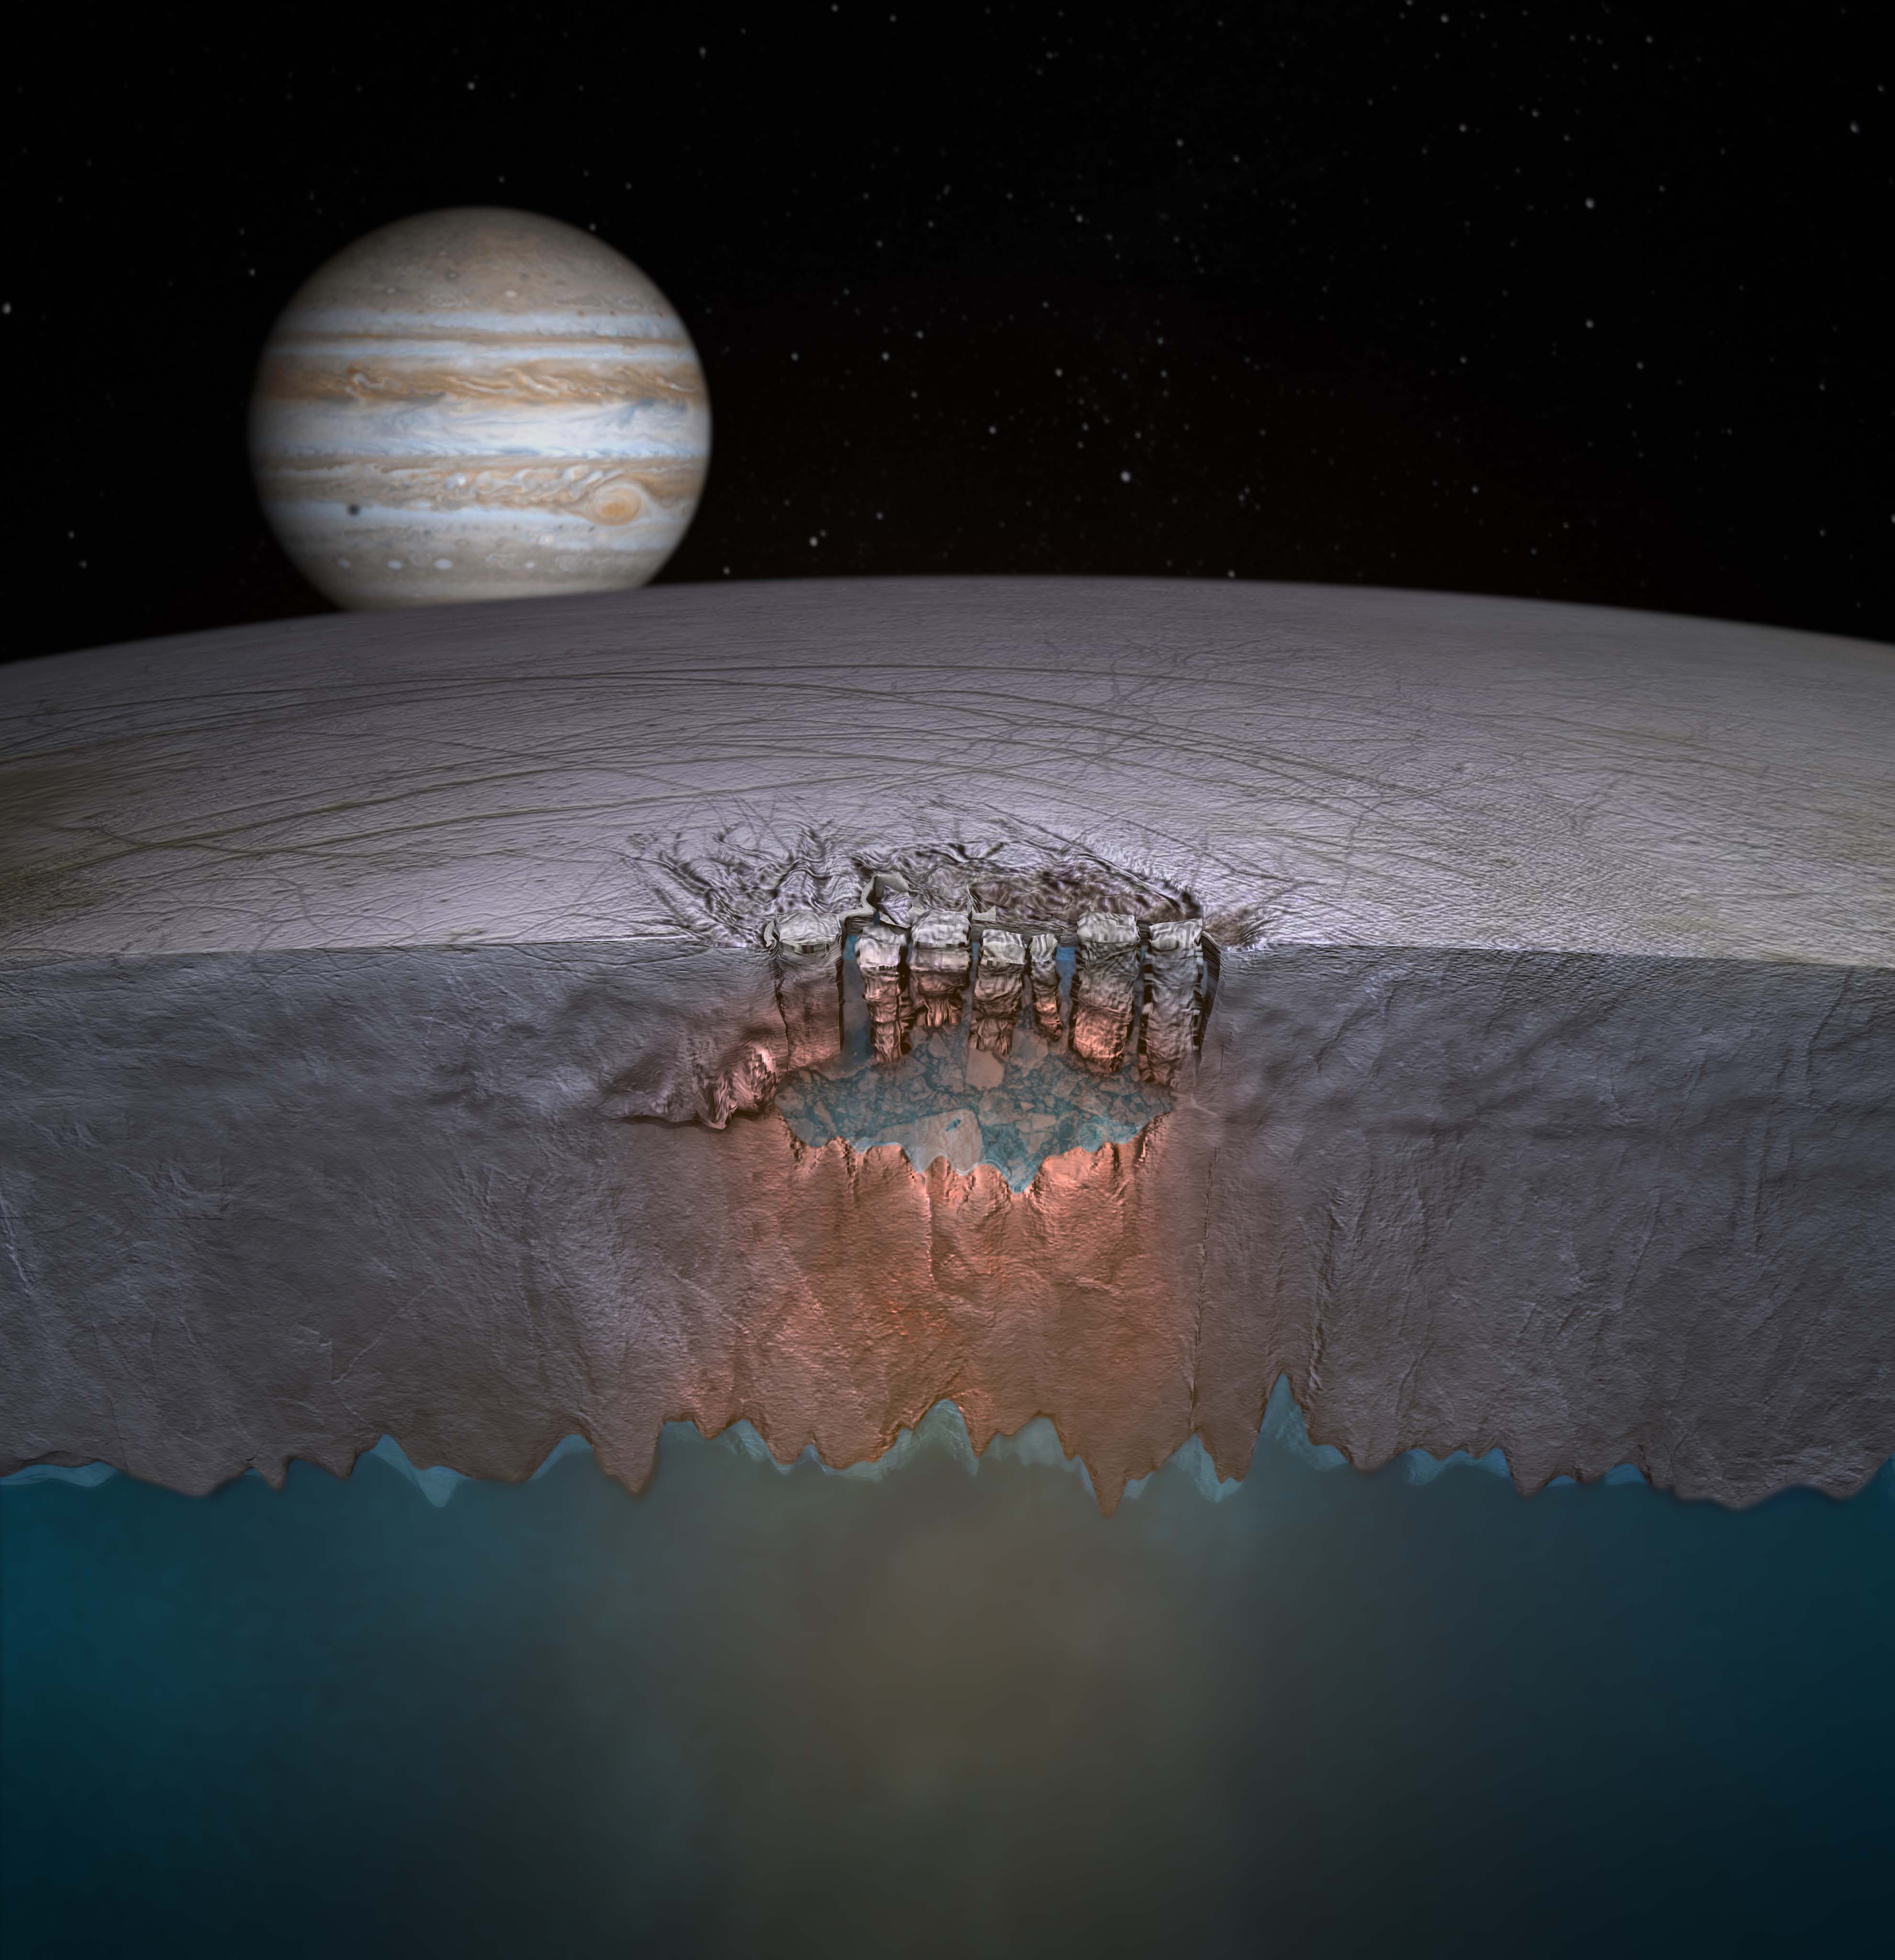
\includegraphics[width=0.5\textwidth]{figures/Rasmus/ArtLake}
	\caption{Artistic illustration of potential water lense, or lake, in the ice shell. \label{fig: ArtLake}}
\end{figure}
As such, apparent "Chaos Regions" has been observed on the surface of Europa and their causes has for a long time alluded scientists. However, recent studies suggests that these are formed due to water lenses in the shell, which can also be interpreted as lakes of liquid water \cite{IceLakes}. They way even be present within $3km$ of the surface, and it is estimated that there may be a water lense consisting of $20,000 - 60,000km^3$ of liquid water beneath the so-called Thera Macula chaos region. An artistic illustration of this phenomenon is shown on fig \ref{fig: ArtLake}.

\iffalse
* Ice thickness

* Composition of the ice? % Se: SWRI: "barr-showman-2009" (ask Kristian Lauszus)

* Lakes?
\fi

\autsubsection{Ice temperature profile}{Kristian Sloth Lauszus}
\label{sec:IceTemperatureProfile}

%* Indirect: salinity, melting speed
%* Drill sample
%* Passive screw in the tip
%	* Thermal isolated
%* Measure heat conductivity of the water
%	* Can be used to estimate the salinity of the water
%		* Melting speed
%
%* "back of the envelope" calculations

In order to estimate the descent time it is important to know the ice temperature profile i.e. the temperature change as a function of the depth and the energy required in order to melt the column of ice. The thermal conductivity of polycrystalline ice can be calculated according to the following equation\cite[(2.3)]{article:thermalConductivity}:
\begin{equation}
	k(T) = \frac{a_1}{T} + a_0
\end{equation}
Where the constants $a_1$ and $a_0$ are given by:
\begin{align}
	a_1 &= \unitfrac[4.88 \e7]{ergs}{cm \, s} \\ \nonumber
		&= \unitfrac[488]{W}{m} \\
	a_0 &= \unitfrac[4.68 \e4]{ergs}{cm \, K \, s} \\ \nonumber
		&= \unitfrac[0.468]{W}{m \, K}
\end{align}
The boundary conditions for the temperature is simply given by 273.15 K at the transition between the water and ice and 100 K at the surface of the moon\cite{article:thermalConductivity}. Thus the temperature difference can be calculated:
\begin{align}
	& T_m = \unit[273.15]{K} \\
	& T_s = \unit[100]{K} \\
	& T_\Delta = T_m - T_s = \unit[173.15]{K}
\end{align}
Figure \ref{fig:T_vs_k} shows two plots of the thermal conductivity as a function of the temperature. Figure \ref{fig:T_vs_k_full} shows the thermal conductivity from 0 K to 273.15 K, figure \ref{fig:T_vs_k_zoom} on the other hand shows only shows the thermal conductivity in the range of the boundary conditions.
\begin{figure}[htb]
	\centering
	\subfloat[From 0 K to 273.15 K]{
		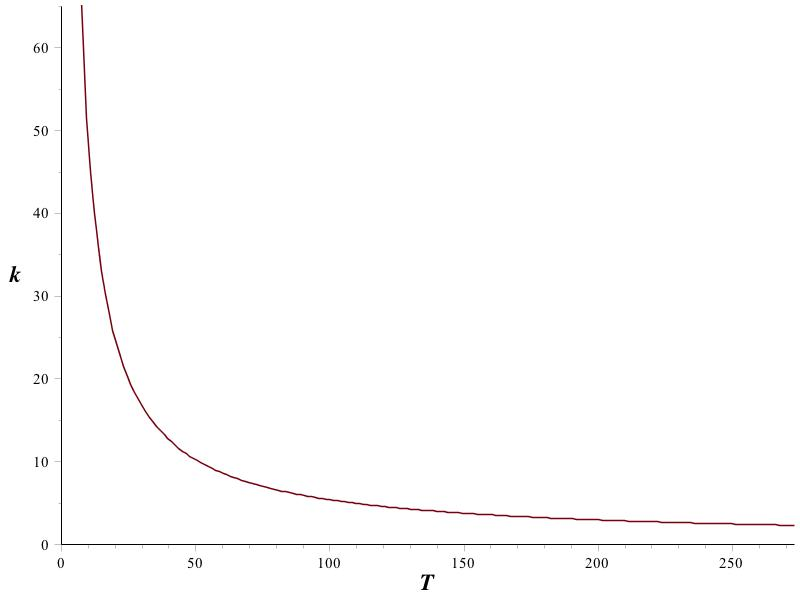
\includegraphics[width=.48\textwidth]{figures/temperature/T_vs_k}
		\label{fig:T_vs_k_full}
	}
	\subfloat[From $T_s$ to $T_m$]{
		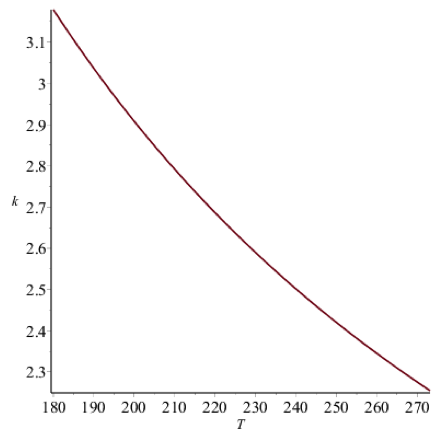
\includegraphics[width=.48\textwidth]{figures/temperature/T_vs_k_zoom}
		\label{fig:T_vs_k_zoom}
	}
	\caption{Thermal conductivity as a function of the temperature}
	\label{fig:T_vs_k}
\end{figure}
The conductive heat transfer can be calculated fairly easily using Fourier's Law\cite{website:conductiveHeatTransfer}:
\begin{align}
	q(T) &= \frac{k(T) A T_\Delta}{d}
\end{align}
The area $A$ is the area of the penetrator facing the ice and by assuming a cylinder with a radius of 10 cm the area is given by:
\begin{align}
	A &= \pi \, 0.1^2 \approx \unit[0.03]{m^2}
\end{align}
Figure \ref{fig:T_vs_q} shows a plot of the conductive heat transfer as a function of the temperature. The thickness of the ice $d$ is assumed to be 3 km according to chapter \ref{sec:structural_profile}.
\begin{figure}[htb]
	\centering
	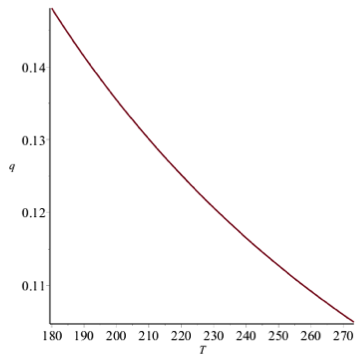
\includegraphics[width=.48\textwidth]{figures/temperature/T_vs_q}
	\caption{Conductive heat transfer as a function of the temperature}
	\label{fig:T_vs_q}
\end{figure}
Notice how both the conductive heat transfer $q$ and the thermal conductivity $k$ are approximately constant doing the interval $T_s$ to $T_m$, thus they can both be approximated by the average over the interval:
\begin{align}
	\bar{k} &= \unitfrac[3.80]{W}{m \, K} \\
	\bar{q} &= \unit[0.0066]{W}
\end{align}
Now the temperature as a function of the depth $d$ can be calculated assuming that the heat transfer and thermal conductivity are constant throughout the ice:
\begin{align}\label{eq:T_d}
	T(d) &= T_s + d \frac{\bar{q}}{\bar{k} A} = 100 K + \unitfrac[0.058 d]{K}{m}
\end{align}
Figure \ref{fig:d_vs_T} shows a plot of the temperature as a function of the depth into the ice.
\begin{figure}[htb]
	\centering
	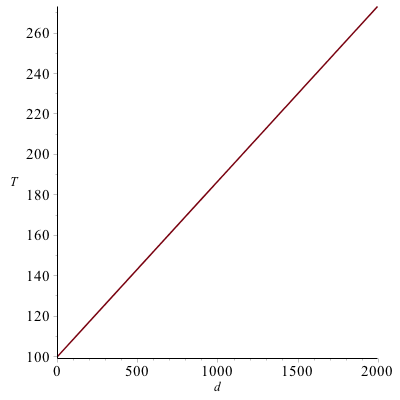
\includegraphics[width=.48\textwidth]{figures/temperature/d_vs_T}
	\caption{Temperature as a function of the depth}
	\label{fig:d_vs_T}
\end{figure}
Figure \ref{fig:T_vs_rho} shows the density of ice as a function of the temperature using the values found in Table \ref{tab:ice_density}. This is be approximated by a linear second order function:
\begin{equation}\label{eq:rho_approx}
	\rho(T) = 931.21 - 0.68 \e{-3} T - 0.19 \e{-3} T^2
\end{equation}
Figure \ref{fig:T_vs_rho_approx} shows a plot of the approximated density of ice as a function of the temperature.
\begin{figure}[htb]
	\centering
	\subfloat[Density of ice according to Table \ref{tab:ice_density}]{
		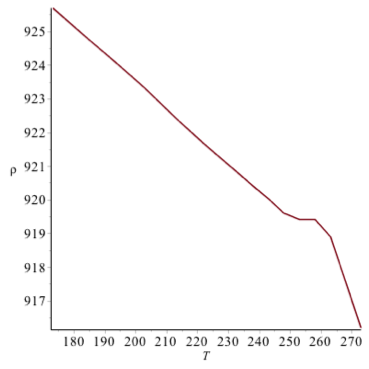
\includegraphics[width=.48\textwidth]{figures/temperature/T_vs_rho}
		\label{fig:T_vs_rho}
	}
	\subfloat[Approximated ice density using \eqref{eq:rho_approx}]{
		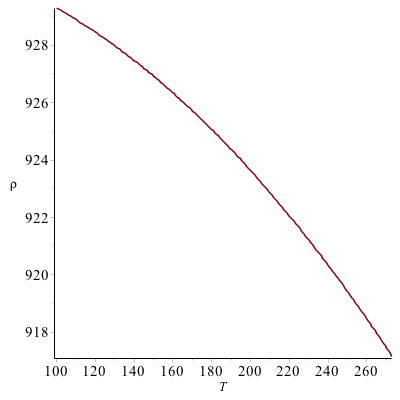
\includegraphics[width=.48\textwidth]{figures/temperature/T_vs_rho_approx}
		\label{fig:T_vs_rho_approx}
	}
	\caption{Density of ice as a function of the temperature}
\end{figure}
\begin{table}[htb]
	\centering
	\resizebox{\textwidth}{!}{%
	\begin{tabular}{|c|c|c|c|c|c|c|c|c|c|c|c|c|c|c|c|}\hline
		$\mathbf{T} ~ (K)$ & 273.15 & 268.15 & 263.15 & 258.15 & 253.15 & 248.15 & 243.15 & 238.15 & 233.15 & 223.15 & 213.15 & 203.15 & 193.15 & 183.15 & 173.15 \\ \hline
		$\mathbf{\rho} ~ (\unitfrac{kg}{m^3})$ & 916.2 & 917.5 & 918.9 & 919.4 & 919.4 & 919.6 & 920.0 & 920.4 & 920.8 & 921.6 & 922.4 & 923.3 & 924.1 & 924.9 & 925.7 \\ \hline
	\end{tabular}}
	\caption{Density of ice for different temperatures\cite{website:iceDensity}}
	\label{tab:ice_density}
\end{table}
Now the density as a function of the distance can be calculated by inserting \eqref{eq:T_d} into \eqref{eq:rho_approx}:
\begin{equation}\label{eq:rho_approx_d}
	\rho(d) = 929.29 - 0.22 \e{-2} d - 6.19 \e{-7} d^2
\end{equation}
%A plot of \eqref{eq:rho_approx_d} and \eqref{eq:T_diff} can be seen in Figure \ref{fig:d_vs_rho} and Figure \ref{fig:d_vs_T_delta} respectively.
%\begin{figure}[htb]
%	\centering
%	\captionsetup[subfigure]{width=0.45\textwidth}
%	\subfloat[Ice density as a function of the depth using \eqref{eq:rho_approx_d}]{
%		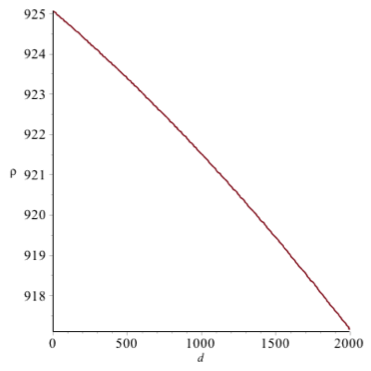
\includegraphics[width=.48\textwidth]{figures/temperature/d_vs_rho}
%		\label{fig:d_vs_rho}
%	}
%	\subfloat[Temperature difference as a function of the depth]{
%		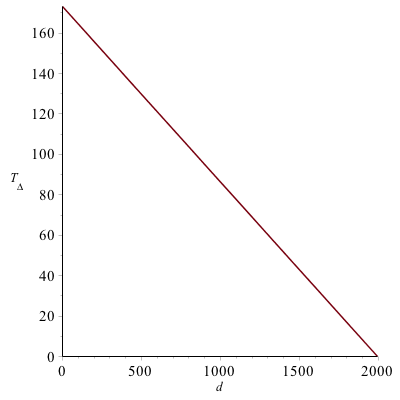
\includegraphics[width=.48\textwidth]{figures/temperature/d_vs_T_delta}
%		\label{fig:d_vs_T_delta}
%	}
%	\caption{}
%\end{figure}
Figure \ref{fig:T_vs_Cice} shows the specific heat capacity of ice plotted using the data found in Table \ref{tab:ice_heat_capacity}. Again this is approximated using a linear second order function:
\begin{equation}\label{eq:Cice_approx}
	C_{ice}(T) = -372.95 + 12.34 T - 0.013 T^2
\end{equation}
The specific heat capacity of ice as a function of the distance can be calculated by inserting \eqref{eq:T_d} into \eqref{eq:Cice_approx}:
\begin{equation}\label{eq:Cice_approx_d}
	C_{ice}(d) = 734.76 + 0.57 d - 0.42 \e{-4} d^2
\end{equation}
A plot of the approximated specific heat capacity can be seen in Figure \ref{fig:T_vs_Cice_approx}.
\begin{figure}[htb]
	\centering
	\subfloat[Specific heat capacity of ice according to Table \ref{tab:ice_heat_capacity}]{
		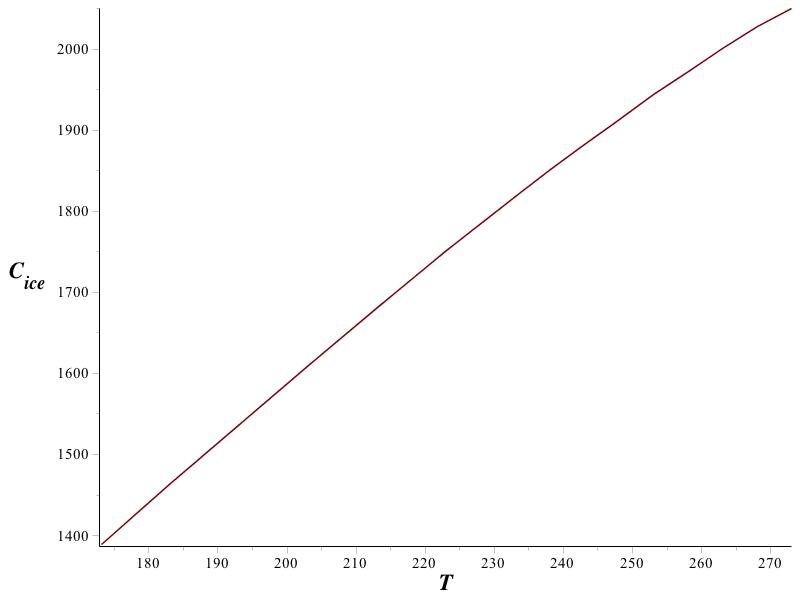
\includegraphics[width=.48\textwidth]{figures/temperature/T_vs_Cice}
		\label{fig:T_vs_Cice}
	}
	\subfloat[Approximated specific heat capacity of ice using \eqref{eq:Cice_approx}]{
		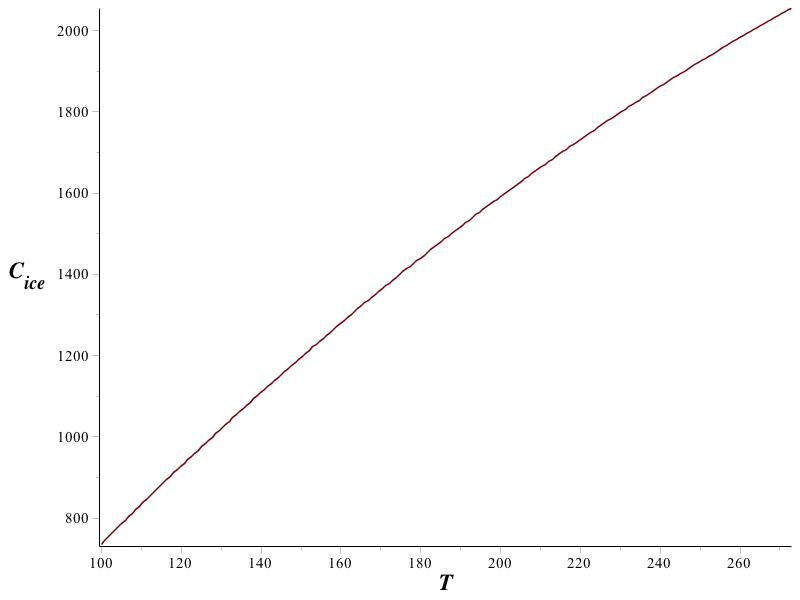
\includegraphics[width=.48\textwidth]{figures/temperature/T_vs_Cice_approx}
		\label{fig:T_vs_Cice_approx}
	}
	\caption{Specific heat capacity of ice as a function of the temperature}
\end{figure}
\begin{table}[htb]
	\centering
	\resizebox{\textwidth}{!}{%
	\begin{tabular}{|c|c|c|c|c|c|c|c|c|c|c|c|c|c|c|c|}\hline
		$\mathbf{T} ~ (K)$ & 273.15 & 268.15 & 263.15 & 258.15 & 253.15 & 248.15 & 243.15 & 238.15 & 233.15 & 223.15 & 213.15 & 203.15 & 193.15 & 183.15 & 173.15 \\ \hline
		$\mathbf{C_{ice}} ~ (\unitfrac{J}{K \, kg})$ & 2050 & 2027 & 2000 & 1972 & 1943 & 1913 & 1882 & 1851 & 1818 & 1751 & 1681 & 1609 & 1536 & 1463 & 1389 \\ \hline
	\end{tabular}}
	\caption{Specific heat capacity of ice for different temperatures\cite{website:iceDensity}}
	\label{tab:ice_heat_capacity}
\end{table}
%\begin{figure}[htb]
%	\centering
%	\includegraphics[width=.48\textwidth]{figures/temperature/d_vs_C_ice}
%	\caption{Specific heat capacity of the depth}
%	\label{fig:d_vs_C_ice}
%\end{figure}
The amount the temperature needs to be raised as a function of the distance is given by:
\begin{equation}\label{eq:T_diff}
	T_\Delta(d) = T_m - T(d) = 173.15 K - \unitfrac[0.058 d]{K}{m}
\end{equation}
The energy required to heat up the 3 km cylinder of ice to 0 \textdegree C can now be calculated:
\begin{align}
	E_0 &= A \, \int_0^{3\e{3}} \! C_{ice}(d) \, \rho(d) \, T_\Delta(d) \ \mathrm{d}d \\ \nonumber
	    &= \unit[8.93 \e{9}]{J}
\end{align}
The total mass of a 3 km cylinder of ice with an area of $A$ is given by:
\begin{equation}\label{eq:ice_total_mass}
	m_{total} = A \, \int_0^{3\e{3}} \! \rho(d) \ \mathrm{d}d = \unit[83174]{kg}
\end{equation}
Latent heat of melting of ice is given by\cite{website:waterLatentHeat}:
\begin{equation}
	L_m = \unitfrac[333.55 \e{3}]{J}{kg}
\end{equation}
The energy required for the phase change can now be calculated:
\begin{equation}
	E_{phase} = L_m m_{total} = \unit[2.77 \e{10}]{J}
\end{equation}
The total amount of energy is then given by:
\begin{equation}\label{eq:E_total}
	E_{total} = E_0 + E_{phase} = \unit[3.67 \e{10}]{J}
\end{equation}
It is noticeable that the energy required for the phase change takes up about 75 \% of the total energy, thus the approximations regarding the thermal conductivity, conductive heat transfer, and heat capacity should not have a huge impact on the result.

However the model of the ice density has a impact on the energy calculations of the phase change, as seen by \eqref{eq:ice_total_mass}. Thus a better model of the ice density would be beneficial. Further studies of the ice composition will be needed in this case, as the ice is assumed to be an isotropic and homogeneous material in the previous calculations. Furthermore the temperature at which the phase change occurs depends on the pressure as well.

It is also noticeable that the energy required to melt the ice will be higher in practice than the total energy calculated in \eqref{eq:E_total}, as their will never be a 100 \% thermal energy transportation efficiency between the melting-device and the ice.
\\
\\
A further study of the ice temperature profile will be presented in chapter \ref{sec:temp_simulation}, which will do a simulation based on the concept introduced in this chapter.

\subsubsection{Pressure Profile}

* What is the outside pressure?

\autsubsection{Water convection}{Kristian Sloth Lauszus}

In this section the concept of natural convection will be presented and CFD (computational fluid dynamics) simulations will be used in order to estimate the natural convection for the penetrator.
\\
\\
Natural convection is interesting as it might be a means of transporting the water from the tip to inside the penetrator passively, guiding the water to the different instruments.  This is needed, as it would be interesting to analyse the salinity and various other elements in the melted water as the penetrator descents. The passive system would eliminate the needs for a pump system, which will add to the complexity and mass of the penetrator.

A sketch of the proposed water transportation system can be seen in Figure \ref{fig:water_transportation}. The intentions is to have the water flow from the intake to the end of the penetrator while running pass the different instruments placed in chambers along the exterior of the penetrator. The flute shape in the tip is intended to guide the water to the intakes in the side. This shape will also be useful in order to guide dirt, small rocks and other small items away from the front of the penetrator, which will improve the heat transfer efficiency between the tip and the ice. Furthermore the screw in the tip, as shown in Figure \ref{fig:water_transportation}, can be used for direct measurement of the temperature of the ice. However it will be important to thermally isolate this from the melter and/or compensate for its effect on the temperature measurement, so the true temperature of the ice can be obtained. Another option would be to have an active screw going into the ice a certain intervals, but the passive system is desirable due to simplicity of this design. % TODO: YouTube video
\begin{figure}[htb]
	\centering
	\captionsetup[subfigure]{width=0.25\textwidth}
	\subfloat[Sketch of the penetrator with flute shape used for dirt removal and water redirection]{
		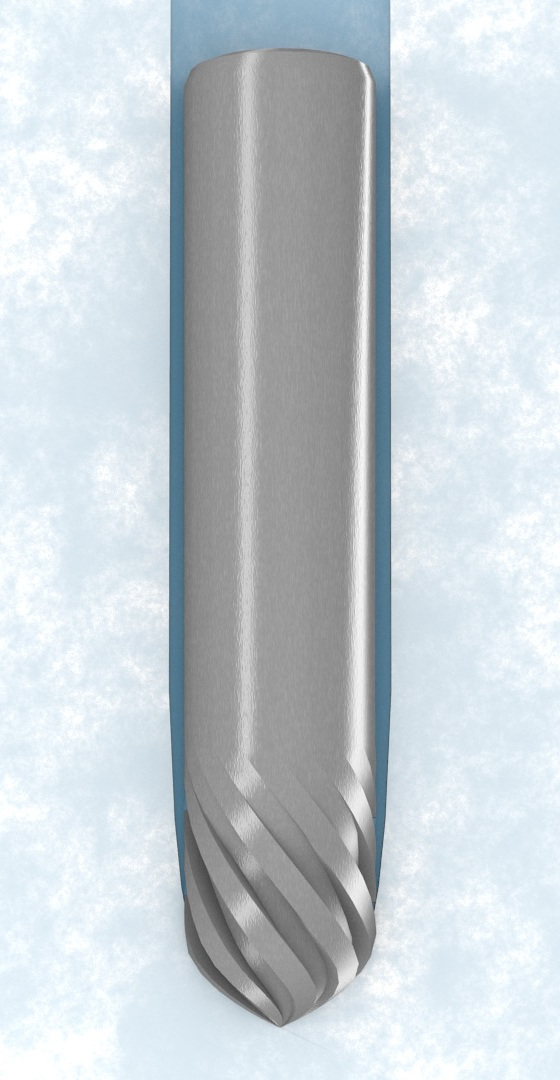
\includegraphics[width=.3\textwidth]{figures/convection/penetrator_model_cropped}
		\label{fig:penetrator_model}
	}
	\subfloat[Cross-section showing the passive water transportation system]{
		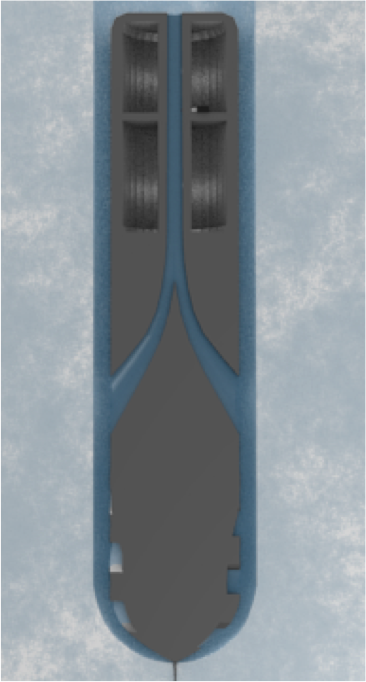
\includegraphics[width=.3\textwidth]{figures/convection/water_transportation}
		\label{fig:water_transportation}
	}
	\caption{Sketch of the penetrator design}
%	\label{fig:}
\end{figure}
\\
Natural convection is caused by density gradients due to temperature differences in a fluid. In this example the water near the tip will be warmer than the water located at behind the penetrator this will cause the less dense water in the bottom to rise with a certain velocity, thus we can take advantage of this effect and redirect the water from the tip to the inside of the penetrator, as explained earlier\cite{website:naturalConvectionPdf}.

An important number associated with natural convection is the so-called Rayleigh number $\mathbf{Ra}$, which is given by\cite{website:naturalConvectionWiki}:
\begin{equation}
	\mathbf{Ra} = \frac{\Delta\rho g L^3}{\alpha \mu}
\end{equation}
If the Rayleigh number is larger than a certain critical value, natural convection occurs. $\Delta\rho$ is the difference in density. It can be approximated using the temperature at the bottom and top of the penetrator and then inserting them into \eqref{eq:rho_approx}. $g$ is the local gravitational acceleration. In this case it is 0.134 g on Europa\cite{website:europaGravity}. $L$ is the characteristic length and can be approximated as the length of the penetrator. This is only an approximation as the water column above will also effect the convection. $\alpha$ and $\mu$ are the thermal diffusivity and dynamic viscosity of the fluid. % Note that the length of the penetrator will have a huge impact on the water flow, as the the Rayleigh number is proportional to the characteristic length third, thus the natural convection can be increased a lot by increasing the length of the penetrator.

% TODO:
	% How to measure melting speed
	% Measure heat conductivity of the water
		% Can be used to estimate salinity - can perhaps be used to estimate the melting speed?

\subsubsection{CFD analysis}

Figure \ref{fig:3d_model} shows a CAD model of the penetrator design. The model was simplified to have a channels having the same effect as the flute resulting in guiding the water into the intakes into the penetrator. However due to the complexity a even simpler model was made, as shows in Figure \ref{fig:simplified_3d_model}. The simplified model simply contains of a heating element in the front of a hollow cylinder surrounded by solid ice along the sides. In the back the water column is simulated infinite long. % TODO: How many watts was the RTG assumed to be?
\begin{figure}[htb]
	\centering
	\subfloat{
		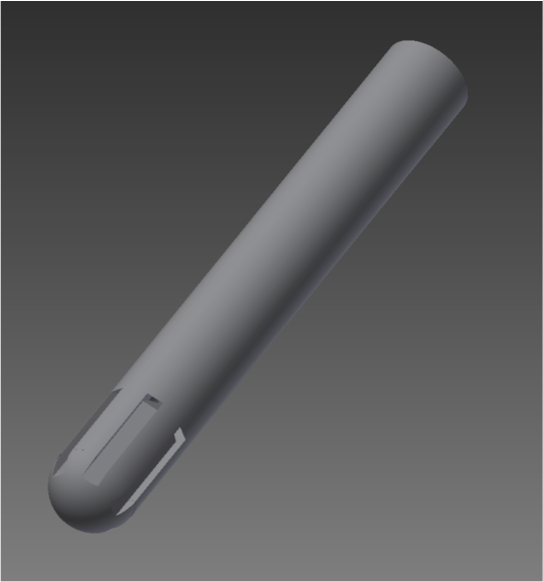
\includegraphics[width=.48\textwidth]{figures/convection/3d_model}
	}\\
	\subfloat{
		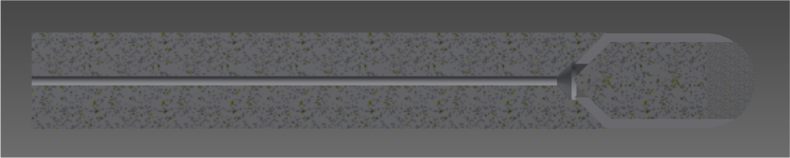
\includegraphics[width=.48\textwidth]{figures/convection/3d_model_inside}
	}
	\caption{3D model of the penetrator design}
	\label{fig:3d_model}
\end{figure}
\\
By using these boundaries conditions and CFD analysis was made, as can be seen in Figure \ref{fig:cfd}. It can be seen the tip gets about 100 \textdegree C. Resulting in a natural convection through the penetrator at only 0.4 cm/s or 200 s/L, thus a pump system such as a peristaltic pump is properly needed, this will be discussed more in detail in chapter \ref{sec:water_flow}.

% TODO: Comment on different assumptions
	% I følge simuleringen så bliver den cirka 100 grader (celsius). Reelt vil det nok være mindre, fordi varmen skal fordeles rundt i hele penetratoren
	% Cirka 10-15 grader, hvis vi følger CFD simuleringen, hvilket passer meget godt med smelte-simuleringen

\begin{figure}[htb]
	\centering
	\subfloat[Simplified 3D model used for CFD analysis]{
		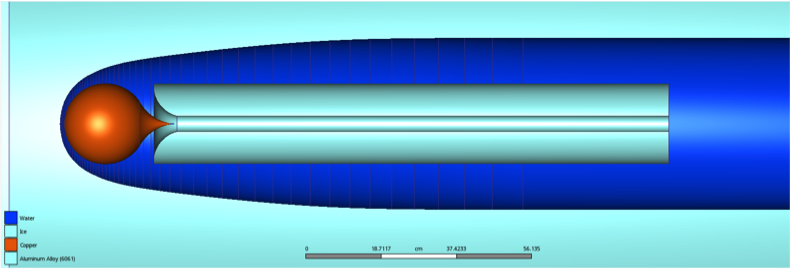
\includegraphics[width=.6\textwidth]{figures/convection/simplified_3d_model}
		\label{fig:simplified_3d_model}
	}\\
	\subfloat[CFD temperature simulation results]{
		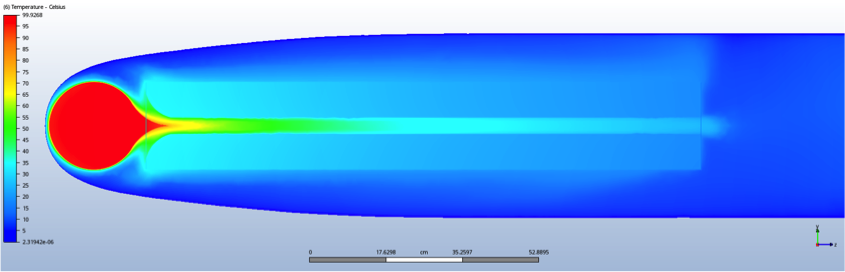
\includegraphics[width=.6\textwidth]{figures/convection/cfd_temperature}
	}\\
	\subfloat[CFD velocity simulation results]{
		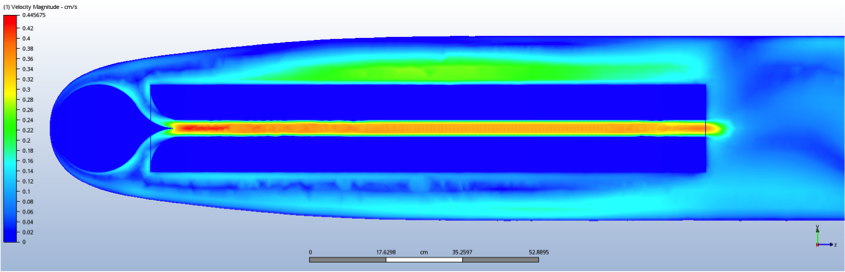
\includegraphics[width=.6\textwidth]{figures/convection/cfd_velocity}
	}
	\caption{CFD simulation results}
	\label{fig:cfd}
\end{figure}


\autsection{Ice Losses}{Nissopoulos Ioannis}
\label{sec:ice_losses}

As we expect, Europa's subsurface consists mainly of several kilometres of ice, which we want to penetrate with electromagnetic waves to establish the communication link between the penetrator and the lander vehicle. Fortunately, a lot of research has been made in the recent decades on how efficient an electromagnetic wave can penetrate different ice layers and on which parameters can affect this propagation. These principles are applied widely in subsurface radar sounding that take place in polar areas, but also in planetary exploration (Mars). For a wide range of frequencies, ranging from MHz to GHz, dielectric losses of ice are independent of frequency. By that it is meant that, the number of wavelengths, which can penetrate into ice before being attenuated to a given fraction of its initial amplitude ($1/e$ of initial amplitude) is approximately the same regardless of frequency. The above implies that the longer the wavelength, the deeper the radar signal can penetrate before being attenuated below the detection of our equipment. Thus, deep ice penetration requires that the radar operates at the lowest possible frequency. 

\paragraph{Dielectric properties of ice}
(For the following two paragraphs \cite{Kofman_2010} has used as main reference.)The permittivity $\epsilon$ of a material is a property describing how much more energy is stored though change separation than in vacuum. Frequency dependence of permittivity occurs because change separation does not happen instantaneously. Changes separate with finite velocities, thus if the external field is reversing polarity too quickly the changes cannot move fast enough to keep up. The frequency at which the charges fully separate and are in constant motion is called the relaxation frequency. At frequencies below the relaxation frequency the permittivity plateaus at the low frequency limit (static) $\epsilon_{s}$, which is often call dielectric constant. At high frequencies above the relaxation frequency the permittivity plateaus at the high frequency limit $\epsilon_{\infty}$. Moreover, ice crystal formation has an impact on polarization, which primarily depends on temperature.

Debye model takes into account the above mentioned theory about dielectric constant of ice and is described by the following equations: 

\begin{equation}
    \epsilon=\epsilon_{\infty}+\Delta \epsilon \frac{\Delta \epsilon}{1+j \omega \tau}
    \label{eq:dielectric}
\end{equation}

, where $\omega = 2\pi f$, $\Delta \epsilon=\epsilon_{s} -\epsilon_{\infty}$ and $\tau$ is the dielectric relaxation time. \\
The permittivity is a complex function of frequency and usually is described by its real and imaginary part.

\begin{equation}
    Re (\epsilon)=\epsilon_{\infty}+\Delta \epsilon \frac{\Delta \epsilon}{1+ \omega^2 \tau^2}
\end{equation}

\begin{equation}
    Im (\epsilon)=\frac{\Delta \epsilon\ \omega\  \tau}{1+ \omega^2 \tau^2}
\end{equation}
The loss tangent (tan $\delta$) is defined by the ratio of these two parts and characterizes the attenuation of the electromagnetic waves in a medium due to ohmic conductivity $\sigma$. 

\begin{equation}
    tan \delta=\frac{Re(\epsilon)}{Im(\epsilon)}=\frac{\sigma}{\omega\ Re(\epsilon)}
    \label{eq:tan}
\end{equation}
The conductivity $\sigma$ of the medium is directly proportional to the imaginary part of the dielectric constant.

Because of the complexity of equations (\ref{eq:dielectric} - \ref{eq:tan}) an approximated expression has been developed to compute the attenuation.

\begin{align}\label{eq:losses}
    a &= 0.129 \sqrt{Re(\epsilon)}\ f (\sqrt{1+tan^2 \delta}-1)^{1/2} \\ \nonumber
      &\approx 0.091 \sqrt{Re(\epsilon)}\ f\ tan \delta \\ \nonumber
      &\approx 0.0009\ \sigma\ dB/m
\end{align}
Where, $\sigma$ is in $\mu S m^{-1}$. As one can see from eq. (\ref{eq:losses}), attenuation's value is directly proportional to frequency, or in other words to the conductivity of the medium. Additionally, the static dielectric constant of pure ice is heavily depended on the orientation of electric field with respect to the crystal's axis. The effect of pressure is about 1\% per kbar for polycrystalline ice \cite{Kofman_2010}. The above formulas and their approximations concerning the electromagnetic waves can be used adequately for very low temperatures, as the ranges we are interested.

Nevertheless, the losses due to pure ice are well documented in bibliography, there is a big gap regarding ice impurities on icy moons. The absence of these data are due to uncertainties and lack of knowledge of the physical nature of impurities on these satellites. This problem was studied by  Moore \cite{Moore_2000} and Chyba \cite{Chyba_1998} for Europa. Moore considered three types of water ice on Europa, produced by three basic processes occurring on Earth. The first one is meteoric ice formed by atmospheric precipitations, sea ice formed by the freezing of water close to the atmospheric interface and marine ice forming beneath ice shelves directly from ocean water. Moore concluded that similar processes are likely to occur on Europa as well, and that the most probable form of ice would be marine ice. In figure \ref{fig:impurities} Moore sums up the attenuation from different type of impurities in ice \cite{Moore_2000}.

\begin{figure}[htb]
\centering
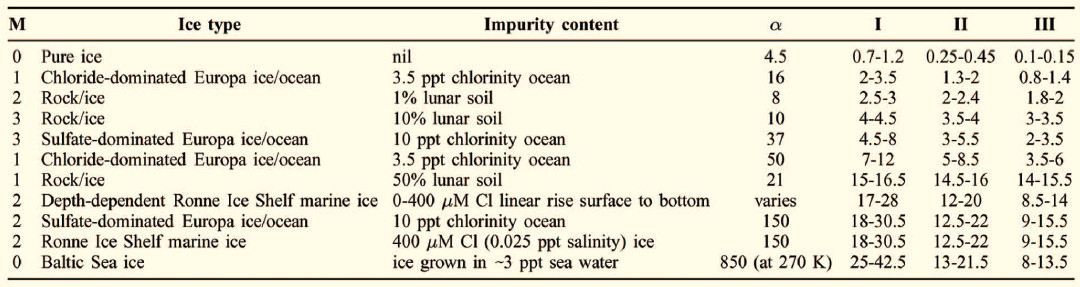
\includegraphics[width=1\textwidth]{figures/Moore2.jpg}
\caption{Attenuation, $a$, is in dB/km at 251 K and corresponds to the one way attenuation due to  ice impurities, in case of a sounding radar. Columns I, II, and III are computed one-way attenuation, in dB/km, for ice shells with base temperatures of 270, 260, and 250 K, respectively. The range of values for each of these corresponds to surface temperatures of 50 and 100 K. These values are independent of shell thickness since the temperature profile is stretched to the ice thickness. The M column represents the plausibility of the ice type for Europa; 0 is least likely while 3 is more likely, given the present understanding
of Europa. The distribution coefficients $k_{0}$ and $k_{MI}$ affecting the marine ice models come from laboratory experiments \cite{Moore_2000}.}
\label{fig:impurities}
\end{figure}
The above calculations data are not taking into account a possible scattering mechanism of electromagnetic wave due to ice layers that can exist in the crust. The scattering effect has a significant impact on the attenuation level and depends strongly on the dimensions of cavities in the medium compared to the wavelength. The two main mechanisms of scattering coming from the ice crust are surface scattering and scattering by volume irregularities. Both these effects can change considerably the penetration depth of the wave into the ice, but also the ratio of any subsurface echo to surface clutter. As we can understand the scattering depends strongly on the wavelength and surface parameters of the body under investigation. 

The conclusion is that the expected one way attenuation because of impurities of ice is in the range 1-8 dB/Km and this number is independent of the frequency. Although, the frequency dependence of attenuation due to scattering mechanisms dictates the use of as low frequencies as possible in order to achieve a deep penetration. The main bottlenecks in that case are two. The first one is that the choice of frequency has an influence on the characteristics of instrumentation and especially on the size of the antenna and the second one is Jupiter's radio emissions spectrum. Figure \ref{fig:J_spec} depicts how Jupiter's activity affect the electromagnetic environment of its moons. Clearly can be seen that frequencies from almost zero Hz up to 50 MHz are dominated from Jupiter's radio emissions. Thus, the exact choice of frequency results in a trade off between science requirements and technical limitations taking into account also the physical constraints of the environment under research. 

\begin{figure}[htb]
\centering
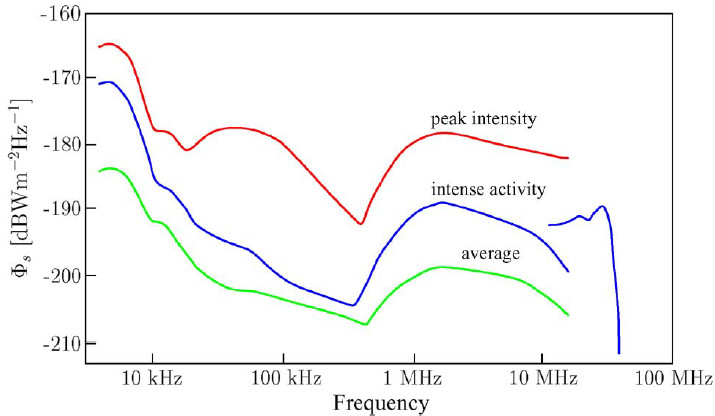
\includegraphics[width=0.7\textwidth]{figures/below100.jpg}
\caption{Jupiter radio spectrum based on Cassini-RPWS data,
normalized to a distance of 1 AU. Green curve: rotation averaged
emission. Blue curve: rotation averaged emission at times of intense
activity. Red curve: peak intensities during active periods. \cite{Grie_meier_2005}}
\label{fig:J_spec}
\end{figure}


\begin{figure}[htb]
\begin{center}
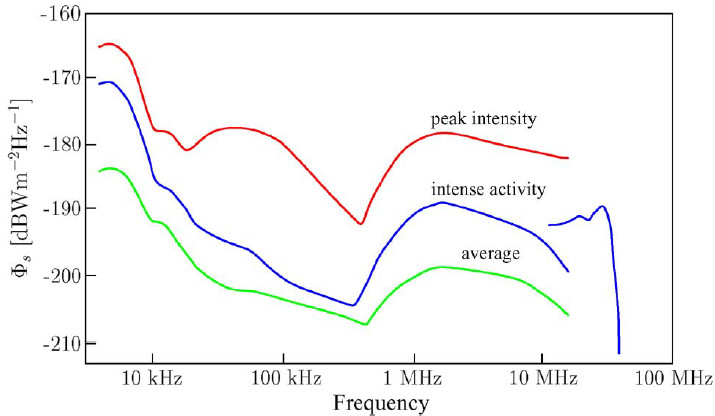
\includegraphics[width=0.7\columnwidth]{figures/below100}
\caption{Replace this text with your caption%
}
\end{center}
\end{figure}

\chapter{Defining Life}

One of the main objectives, if not the main objective, on this mission is to search for life. This is after all a life finding mission and therefore the instrument suite onboard needs to be focused on finding life. The mission is going to look for life in the ice and mostly in the water below the ice, where there is a high expectancy to find some sort of life or life harbouring conditions. \par
Life can be found in many forms and stages of evolution, and it can therefore be very difficult to detect, because we do not know exactly what the penetrator should look for. Before looking into what we should look for on Europa, a set of guide rules needs to be put in place, defining what life forms are already known from earth. It would be ideal to set up a precise yardstick for life, a list of things needed to say that life will exist, but this is not possible. What is possible is to look at what is present on Earth and applying this to alien life forms. \par
Most living organisms as we know from Earth have some properties in common, though non-living matter show some of them, only living organisms show all of them\footnote{$https://da.khanacademy.org/science/biology/intro-to-biology/what-is-biology/a/what-is-life$ 22-05-2016}. The 7 properties are: \par

\begin{enumerate}
  \item Organization
  \item Metabolism
  \item Homeostasis
  \item Growth
  \item Reproduction
  \item Response
  \item Evolution
\end{enumerate}

Beginning at number one “Organization”, to have life, structure is needed, and by taking unorganized matter and organizing it, is a sign of life. Living organisms a made up of one or more cells which in them self are highly organized, and able to produce complex chemical processes from an unorganized energy source. For bigger multi-cell organisms, organization is important, since individual cells are assigned different specific jobs to create a bigger and more complex organism. \par  
Metabolism is the life sustaining chemical transformations happening within cells and living organisms, and is the sum of all chemical reactions happening in a living organism. This chemical conversion can be divided into two subcategories, catabolism and anabolism. Catabolism is the process of breaking down organic matter into energy, with anabolism being the reverse process, building up complex molecules such as protein from simple molecules. This type of process uses energy. One of the most important metabolisms, is the citric acid cycle (Krebs cycle), it is believed to be one of the early established components for cellular metabolism. \par
Most living cells and organisms have a working area where they are able to sustain life; humans need to stay a cool 37 degrees to function normally. The ability to maintain a stable internal environment, even with a varying external environment is called homeostasis. This type of process is mostly found in more complex organisms, like smaller animals. Microorganisms usually depend on their surroundings to create a stable living environment.\par
The fourth properties is growth, this begins at a cellular level and is linked to the organization of the cells in defined structures. It depends on the anabolism to crate proteins and amino acids for DNA. Without growth more complex molecules and organisms would not exist.\par
Reproduction is also important for sustained life, looking at single cell organism like bacteria, which is able to reproduce by simply splitting in two. Reproduction can also take place with two parent organisms creating a new cell from a combination of both their genetic information. 
Organisms need to respond to actions from their environment to be able to survive. That is way many plants turn towards the sun, and bacteria cluster together around a nutrient rich area. When provoking a living organism, heating it, burning it, a response should be detected. It does not need to be movement, it could also be creating a toxin release or other chemical, helping it defend or survive from an unknown threat. \par
Lastly it needs to evolve, their genetics needs to adapt to changes, making it stronger and able to survive. Here natural selection is involved, where traits which make it easier to survive are carried through, by the death of the weaker organism that did not evolve. This is of cause a very slow process, but might be the key to discovering life on other planets, due to its adaptability.\par
These 7 properties of life are all found in living organisms on earth, this does not mean that the yard stick for life is defined perfectly, it is not! It is still hard to define life exact, and this only guides us some of the way. An example of where this does not hold true is for a mule, it is very much alive but is not able to reproduce\footnote{$https://en.wikipedia.org/wiki/Mule$ 22-05-2016}. \par
The properties can give an idea of what to look for when doing analysis of samples from Europa, because some of the processes create by-products that could be detected. One of the most well known processes with this ability is photosynthesis, taking CO2 and energy to create sugar and oxygen. It takes the suns energy and harvests it into chemical energy which can be used as fuel for the organisms. This type of process is very unlikely to take place in the ice or water of Europa, since the sun is 780 million kilometres away, and no light will get through the ice and down in the ocean. In general life needs to be rethought for the Europan environment.  \par
A good place to start the search for life is at the building block level, and looking for process that needs a source of energy, most likely heat, and some chemicals/nutrients, to create sustained life. This type of process is called abiogenesis\footnote{$https://en.wikipedia.org/wiki/Abiogenesis$ 22-05-2016} and is the natural process of living organisms arising from non living matter. The search could therefore go into look for simple non living matter such as simple organic compounds. This will narrow the search down to looking for molecules containing carbon, like in simple carbohydrates, this is of cause just one basic assumption for life, the other obvious one is the energy. No sunlight is reaching the ocean so energy must be created differently, by gravity or thermal activity in the rock core, this will be investigates further in the next chapters. \par
If the energy is there and some simple organic compounds can be found, life might be able to exist. The search therefore need to be increased to look for more complex molecules, here the organization property comes to play.  Now the search for proteins, and single celled organism, like bacteria would be possible living organisms.\par
This would go on, into bacteria colonies and even more complex organisms, but the conclusion is that we need some simple organic building blocks and energy to create some sort of life here on Earth (important distinction). Making a more generalized plan for what life is some other aspects needs to be taking into account by looking even further back to the origin of life.

\subsection{Hypotheses about the origin of life on Earth}
This is one of the difficult ones, because sciences do not know for sure how life came to be, but some important hypotheses have been made around where and how life on Earth originated from. \par
Life on Earth started some 3.5 billion years ago, the evidence for this is found in rock structures around the world, as small fossils of microbes. One place this is still evident today is in stromatolites which are produced by microbes by photosynthesis. They form a layer of microbial film, trapping mud under it, creating lay upon layer of mud and microbes, some dating back to 3.5 billion years ago. \par
The earliest signs of life are found on land, the main hypothesis to where life originates from is in the oceans, more specific the thermal vents on the deep sea ocean floor. The conditions found around these black smokers are ideal for an abiogenesis, due to the chemicals present and the energy in form of heat from the vents. DNA sequencing also suggest that some of the early life was microorganisms living in an aquatic high temperature environment. \par
As talked about in the previous chapter, life is complex, even on a microbe/bacteria level. These complex cells did not just show up, they evolved through small steps and natural selection. Hypotheses to how these more complex multi-celled organisms came to be can be split up in to 5 steps: \par

\begin{enumerate}
  \item In the beginning of Earth life, the atmosphere consisted of nitrogen, hydrogen, ammonia, water vapor and methane. This was able to combine in to simple organic matter, such as nucleotides found in RNA and DNA.
  
  \item The foundation was now set, and next came self replication molecules. These molecules are chains of nucleotides, and are able to replicate them self by some sort of RNA self-replicator process. With self-replicating came also natural selection, not all replications went well, and therefore some survive better than others. This process continued creating more and more stable and efficient replication processes.
  
  \item These replicating cells then got enclosed in a cell membrane, protection the self-replication molecules, these cells had a great advantages over the non enclosed cells, due to the protection of the internal environment from the outside environment.
  
  \item All of this was based on RNA-processes, but when some cells evolved to use DNA, things changed. Now instead of RNA doing the whole replication process, DNA became the genetic material, it is also more stabile then RNA, proteins became responsible for metabolism inside the cell and RNA now only did the part of carrying information from the DNA to the protein building areas of the cell. Below is a figure explaining the new replication process.

\begin{figure}[H]
\caption{The RNA is now the message carrier, and the DNA became the genetic material}
\centering
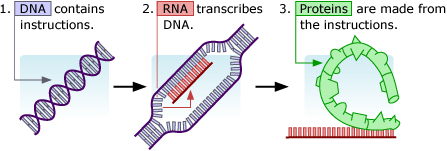
\includegraphics[scale=1]{figures/Agge/dnarnaprotein.png} 
\end{figure}
  
  \item Instead of the cells always splitting up after self replication, some stated to form more complex multi-celled organisms, the beginning of multi-cellular organisms.
\end{enumerate} \par

This was a short investigation into how life on earth could have evolved. Some of the hypotheses are still investigated and some gaps are still to be filled. An example of this is how RNA and proteins where created, because nucleic acids for DNA and RNA productions depend on proteins, but to build proteins nucleic acids are needed. The solution to this problem was first recently discovered, where the knowledge on RNA was expanded, and is was discovered that RNA is able to both store and copy itself concluding that nucleic acids came first \footnote{$http://evolution.berkeley.edu/evolibrary/article/side-0-0/origsoflife-01$24-05-2016}. \par

Many of these processes are dependent on energy from the sun, and it was after the first stromatolites and their photosynthesis the atmosphere started changing and became more oxygen rich. This will have worked as a toxic gas on some anaerobic cells, making aerobic cells more common on land. This just shows how many factors play a role on how life originated and further evolved, killing the first evidence of life as other life forms evolved.\par
From all of this a conclusion can be drawn in what might be expected to be found on Europa, a uplifting clue is found in the black smokers on Earth, which could be found on the bottom of Europa. But from what we see on earth, the most likely life forms are bacteria, or simple multi-cellular life forms, and what we need to look for includes, simple organic compounds, such as carbohydrates, enzymes, lipids fatty acids, nucleic acids, proteins, peptides, amino acids are some of the important compounds which could indicate life or a habitat for life.\par  
Another way to investigate life, is to look at the environment it is created from/in, and if life did exists we might see reminisce of life. The next two chapters look into the life harboring conditions and possible clues to look for from extinct life forms. \par

\subsection{Life harboring conditions and planetary habitability}
This chapter will look into the condition need for life to evolve on a planet, and since life beyond Earth is unknown, the theories on planetary habitability are built on what is known from Earth.\par
Planetary habitability, is a measure of a planet’s ability to harbour life in a habitable environment\footnote{$https://en.wikipedia.org/wiki/Planetary_habitability$ 24-05-2016}, this does not mean that life exists on the planet in question, but just that the conditions are right for life to develop, or to be transferred from another planet.\par 
Some of the requirement for life has already been discussed previously, but show up again in this chapter. One of them is energy, there need to be some sort of energy present, apart from that many other geophysical and astrophysical criteria must be just right, for a planet, to be habitable. Looking at one of NASA’s guide rules for life is “extend regions of liquid water\footnote{$http://www.nasa.gov/jpl/the-solar-system-and-beyond-is-awash-in-water$ 24-05-2016}”  since this is a great place for organic matter to form from, and here energy can come from either the sun in the top ocean layers, or for example black smokers on the bottom.\par
Habitability is not only dependent on the planets environment, atmosphere and so on, but also other externals needs to be considered; here we need to look at the astrophysical properties such as orbit and placement compared to the sun. In all there are many aspects to take in to account and like the chapter about “Defining life” some properties for habitability of a planet can be made:\par

\begin{enumerate}
\item Mass

\item Orbit and rotation

\item Geochemistry

\item Microenvironments and extremophiles

\end{enumerate} \par

The mass of a planet is important to sustaining an atmosphere; this is not a problem on Europa since the life is not expected to be found in its thin atmosphere. With smaller planets the energy left over from creation is lost faster making the planet geologically dead, this is a problem, since life is so dependent on an energy source. In the case of Europa the mass is very little compared to Earth which might point to a geological dead planet, and the energy must therefore come from the ice or the gravitational pull of Jupiter. But this does not always hold true, look at Jupiter’s other moon Io, is geological active, and even with its little mass. This activity comes from the gravity pull from Jupiter. \par
In the orbit stability is key; a stable orbit gives stability to the environment on the planet. The speed of rotation and how elliptic the orbit is, influences the temperatures on the planet, here stable temperatures are favorable, so half the planet is not frozen half the year and boiled the next half year. Looking at Europa the problem is not that impotent, since if life is found, it is located in the water protected by the sounding ice. \par
The geochemistry tells if the fundamental building blocks are present to create the “food” for living organisms. The four important elements from know from Earth are nitrogen, hydrogen, carbon and oxygen. It was already discussed in the chapter about life origin why these are important.  It is hard to tell if these are present in the ocean on Europa, a NASA study describe the “Why look at Europa” describes how hydrogen and oxygen might be present in just the right quantities.\par

When looking at a new planet maybe only a small part of it is habitable, comparing with Earth 3.5 billion years ago, life was not as abundant as it is now. Therefore a small sample from Earth would not have shown any sign of life, even if there was in some extreme place such as at the black smokers on the ocean floor. On Earth organisms know as extremophiles live in these very niche environments with conditions not suitable for “normal” life, there can be temperatures above 100 degrees Celsius, or very acidic/alkaline conditions. This expands the possibility of finding life in more extreme environments such as on Europa. \par
All of this can be summarized in a list of factors; the list was originally made for reproducing and survival of Earth microbes on Mars. The list has been modified to match an environment with no atmosphere\footnote{$http://mepag.jpl.nasa.gov/reports/MEPAG-SR-SAG-final1.pdf$ page 17 24-05-2016}.

\begin{itemize}
   \item  Water availability and activity
   \begin{itemize}
     \item  Activity of liquid water
     \item Past/further liquid (ice)
     \item Salinity and pH
    \end{itemize}
   \end{itemize}
   
     \begin{itemize}
       \item  Chemical environment
       
       \begin{itemize}
         \item Nutrients 
         
         \begin{itemize}
          \item C, H, N, O, P, S, essential metals and micronutrients
          \item Fixed nitrogen
          \item Their availability/mineralogy
         \end{itemize}
          
         \item Toxin
          \begin{itemize}
           \item Heavy metals (Zn, Ni, Cu, Cr, As, Cd, ect.
           \item Globally distributed oxidizing soils
          \end{itemize}
          
       \end{itemize}
     \end{itemize}
     
     \begin{itemize}
       \item  Energy for metabolisms 
       
       \begin{itemize}
         \item Solar/Radiation 
         \item Geochemical
         
         \begin{itemize}
          \item Oxidants
          \item Reductants
          \item Redox processes
         \end{itemize}
          
       \end{itemize}
     \end{itemize}
     
     \begin{itemize}
       \item  Physical condition 
       
       \begin{itemize}
         \item Temperature 
         \item Small temperature fluctuations
         \item High CO2 concentrations
         \item Water/ice flow
           
       \end{itemize}
     \end{itemize}
   
This list gives a good yard stick for determining if the planet is habitable, when Earth life forms are considered. Of cause life could be of a whole other unknown type which today’s technology cannot detect and this will give problems which is left out of this discussion. \par

\subsection{Extinct life}
Due to the small size of Europa, it might be geologically dead, but life might have thrived when the planet still had left over energy from its creation. Therefore it would be an idea to look for signs of extinct life, as we also see from Earth, previous life literally fuels today’s world. \par
When look for extinct life the search for distinct bio-makers/features that would indicate that life once thrived here. The things too look for will be leftovers from living organisms, this includes reduced carbon and nitrogen (CO3(2-), NO3-, NO2-, SO4(-2), also some important metals would be of interest Mg, Mn and Fe. But some of these compounds might not come from extinct life and it is therefore important to distinguish between biologically and not biologically produced compounds. An example of this is seen in the way N2 is deposited, with no biological processes the N2 would become NO2- and NO3-, but if this is used on a biological process it would form N2O or N2 as a gas  (dependent on pressure)\footnote{http://www.ncbi.nlm.nih.gov/pubmed/11537366 25-05-2016}. \par
From earth we see the extinct life in great quantizes such as olie and natural gas, produced by decomposing plants and animal matter under high heat and pressure. Natural gas is mainly made up of methane which would be a good marker for primordial life. Also olies floating on the water would indicate extinct life. \par

Through the last few chapters discussions about what life is and some of the signs to look out for have been investigated. Some of the findings have been applied to Europa and how it might fit the criteria as a life harbouring moon. In the last chapter a discussion about why Europa could be the place to go, for finding alien life in our solar system.\par

\subsection{Why look at Europa}

One of the most important properties of Europa is the liquid water found under the ice, which is key to life according to NASA, the more questionable, but just as important, is the energy need to create and sustain life. As discussed due to the small mass of Europa it might not be geologically active, if this is the case then a new NASA study carried out by JPL\footnote{$http://www.jpl.nasa.gov/news/news.php?feature=6514$ 25-05-2016} show that even without volcanic activity such as hydrothermal vents/black smokers, the balance of chemical energy might be there to support life. The study is based on methods know from Earth, and look at how energy and nutrients are carried around Earth’s oceans. But most importantly how the production of hydrogen and oxygen will take place without volcanic activity, one of the methods fro creating oxygen is serpentinization, where water reacts with freshly exposed rock (cracks form when cooling or water movement) to produce hydrogen. \par
The other part of the study looks in to the production of oxidants and oxygen, here the radiation from Jupiter splits ice/water on the surface, which cycles into the ice and down to the ocean. Scientist does believe that compounds from the top ice slowly cycles through the icy surface. If the amount of oxidants and hydrogen produced Europa is balnced just right, it might have just the right conditions to sustain life. \par
It is already know that Io has volcanic activity due to the Jupiter’s gravity push and pull on the rocky moon. This could indicate volcanic activity on Europa, giving even better conditions for life, due to the energy volcanic activity would bring. If Europa is geologically active there is a good chance of finding black smokers on the seafloor, this is one very important niche environment where life would thrive on the energy source and nutrients the black smokers produce.\par
Europa therefore seems like a perfect place to look for life and is also classified as a class III habitat. A planet in class III has liquid water of some sort trapped in or by ice, but since the water is enclosed the nutrient might be found in too small concentration to contain living organisms. This is the main problem with class III planet/moon, the lack of ingredients for life in one location due to the large water body and therefore lack of an incubator for life with the right amount of nutrients. \par
A illustration of all the possible methods for life to form is showed in the picture below, here radiation, ice cycle and volcanic activity would lead to a possible habitat for life in the ocean of Europa:\par

\begin{figure}[H]
\caption{The different process that Europa might have for producing a habitat for life}
\centering
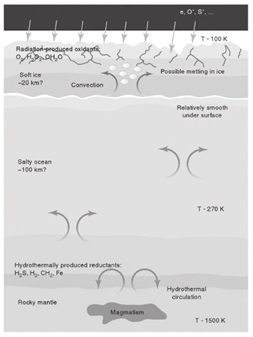
\includegraphics[scale=1]{figures/Agge/Europasurface.png} 
\end{figure}

In conclusion life is very complex to quantify and only a set of guidelines can be set up, derived from the life known to Earth. The guidelines set up give an indication of what to look for, when searching for a habitat or life on another planet, it also points to more precise investigations into what life forms might be found on Europa. It is still difficult to say anything exact of what could be expected to be found on Europa, in form of geology and energy source, but throughout this study it is evident that Europa is a good place the search for life in our solar system. In all Europa ticks many of the right boxes set up for a habitable moon with nutrition and energy to sustain life.


%added theory (Johannes Linde)
\section{Imaging Systems}
%\autsubsection{Telescopes and Cameras}{Johannes Linde}
%\todo[inline]{Types of telescopes etc.}
\autsubsection{Calculating Ground Resolution}{Johannes Linde}\label{sec:ground_res}
To get the required resolution, a specific focal length is required. The focal length can be related to the field of view\footnote{Also known as the angle of view} by equation \eqref{eq:focal_len_fieldofview}. See \cite{wiki_aov2016} for derivation of this equation.
\begin{equation}
\label{eq:focal_len_fieldofview}
\alpha = 2\arctan{\frac{d}{2f}}
\end{equation}
where $d$ represents the sensor size in either the horizontal or vertical direction.

To relate the ground resolution with the field of view, it is necessary to consider the horizontal and vertical view seen by the camera. By applying simple trigonometry, the ground resolution can be described by the distance from the object and the field of view. This is illustrated in figure \ref{fig:angle_of_view_def}.
\begin{figure}[htb]
\centering
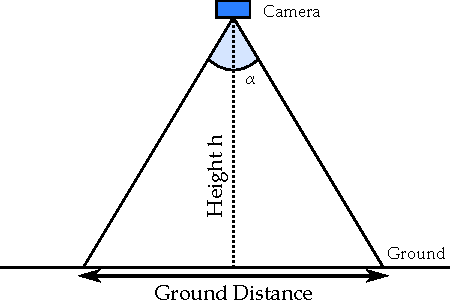
\includegraphics[width=0.65\textwidth]{figures/Orbiter/imaging_angle_of_view}
\caption{Definition of the angle of view. Adapted from:\cite{dsil2014}.}
\label{fig:angle_of_view_def}
\end{figure}
From this figure, it can be seen how the tangent of half the angle of view is equal to the half the ratio between the ground distance and the height. This applies to both the horizontal and vertical distance. If the sensor is not square, the angle and therefore the distance will be different.
\begin{equation}
\label{eq:angle_of_view}
\tan{\frac{\alpha_x}{2}} = \frac{x}{2h}
\end{equation}
By arranging the two equations, the ground distance is defined:
\begin{equation}
\label{eq:ground_dist}
dist_x = 2h\cdot \tan{\frac{\alpha_x}{2}}
\end{equation}
The ground distance defines the total distance covered, when the contributions from all pixels are added together. Therefore, the ground distance per pixel ($\mu_x$ or $\mu_y$)is easily found when the sensor resolution is known. This can be seen in equation \eqref{eq:ground_dist_pixel}:
\begin{equation}
\label{eq:ground_dist_pixel}
\mu_x = \frac{x}{r_x} = 2h\cdot \tan{\frac{\alpha_x}{2}}
\end{equation}
By solving for the the field of view using \eqref{eq:ground_dist}, the focal length can be found using equation \eqref{eq:focal_len_fieldofview}. This applies to both the horizontal and vertical direction, if the sensor is not square.
\begin{equation}
\label{eq:angle_of_view_ground_dist}
\alpha_x = 2h\cdot \tan{\frac{dist_x}{2}}
\end{equation}
The focal length can then be calculated by solving for the focal length in equation \eqref{eq:focal_length_angle_of_view} and using the horizontal or vertical sensor size as $d$.
\begin{equation}
\label{eq:focal_length_angle_of_view}
f = 0.5\cdot\frac{d}{\tan{\left(0.5\cdot \alpha\right)}}
\end{equation}
\subsection{Camera Basics}
\todo[inline]{pinhole camera basics}
\todo[inline]{ccd, cmos difference}
\subsection{Telescope Systems}
\todo[inline]{Types of imagers etc.}
%\section{Spectroscopy}
%\todo[inline]{See power point presentation}
%\section{Europa Surface Environment}
%\todo[inline]{Moon Environment (Radiation etc)}
%\section{Calibrating the Geo-localization System}
%\todo[inline]{How to calibrate (point at Jupiter, get transfer matrix using star trackers)}
%\section{Protecting from radiation}
%\todo[inline]{How to protect from radiation. Dynamic Response to Radiation (Julia)}
%\section{High Gate Measurement}
%\todo[inline]{High Gate Measurement (Operating at very far distance, to track trajectory)}

%added theory
\autsection{Autonomous Landing Site Selection}{Kristian Sloth Lauszus}\label{sec:aut_landing}
%\autsubsection{Image Recognition}{Kristian Sloth Lauszus}
Since the bandwidth from the orbiter to the earth is limited it is beneficial to have a semi-autonomous system that can pick an potential landing site from some given parameters. For instance it would be useful to pick a landing site that does not have any ridges, as there is risk of the lander tipping over after the landing. This could be done by simple edge detection, such as a Laplacian Gaussian filter from a greyscale image. If the system finds a potential landing site the image could then be streamed back to earth either as a binary, greyscale or even the full color image for further analysis. Furthermore object detection could be used to locate certain characteristics. The image could then be cropped and streamed back to earth, thus decreasing the needed bandwidth.

Figure \ref{fig:edge_detection} shows two examples of how a Laplacian Gaussian filter has been used for edge detection on images from the moon. It shows clearly how cracks on the surface show up. These locations could then be picked as potential landing sites and further analysed by the ground control.

\begin{figure}[htb]
	\centering
	\subfloat{
		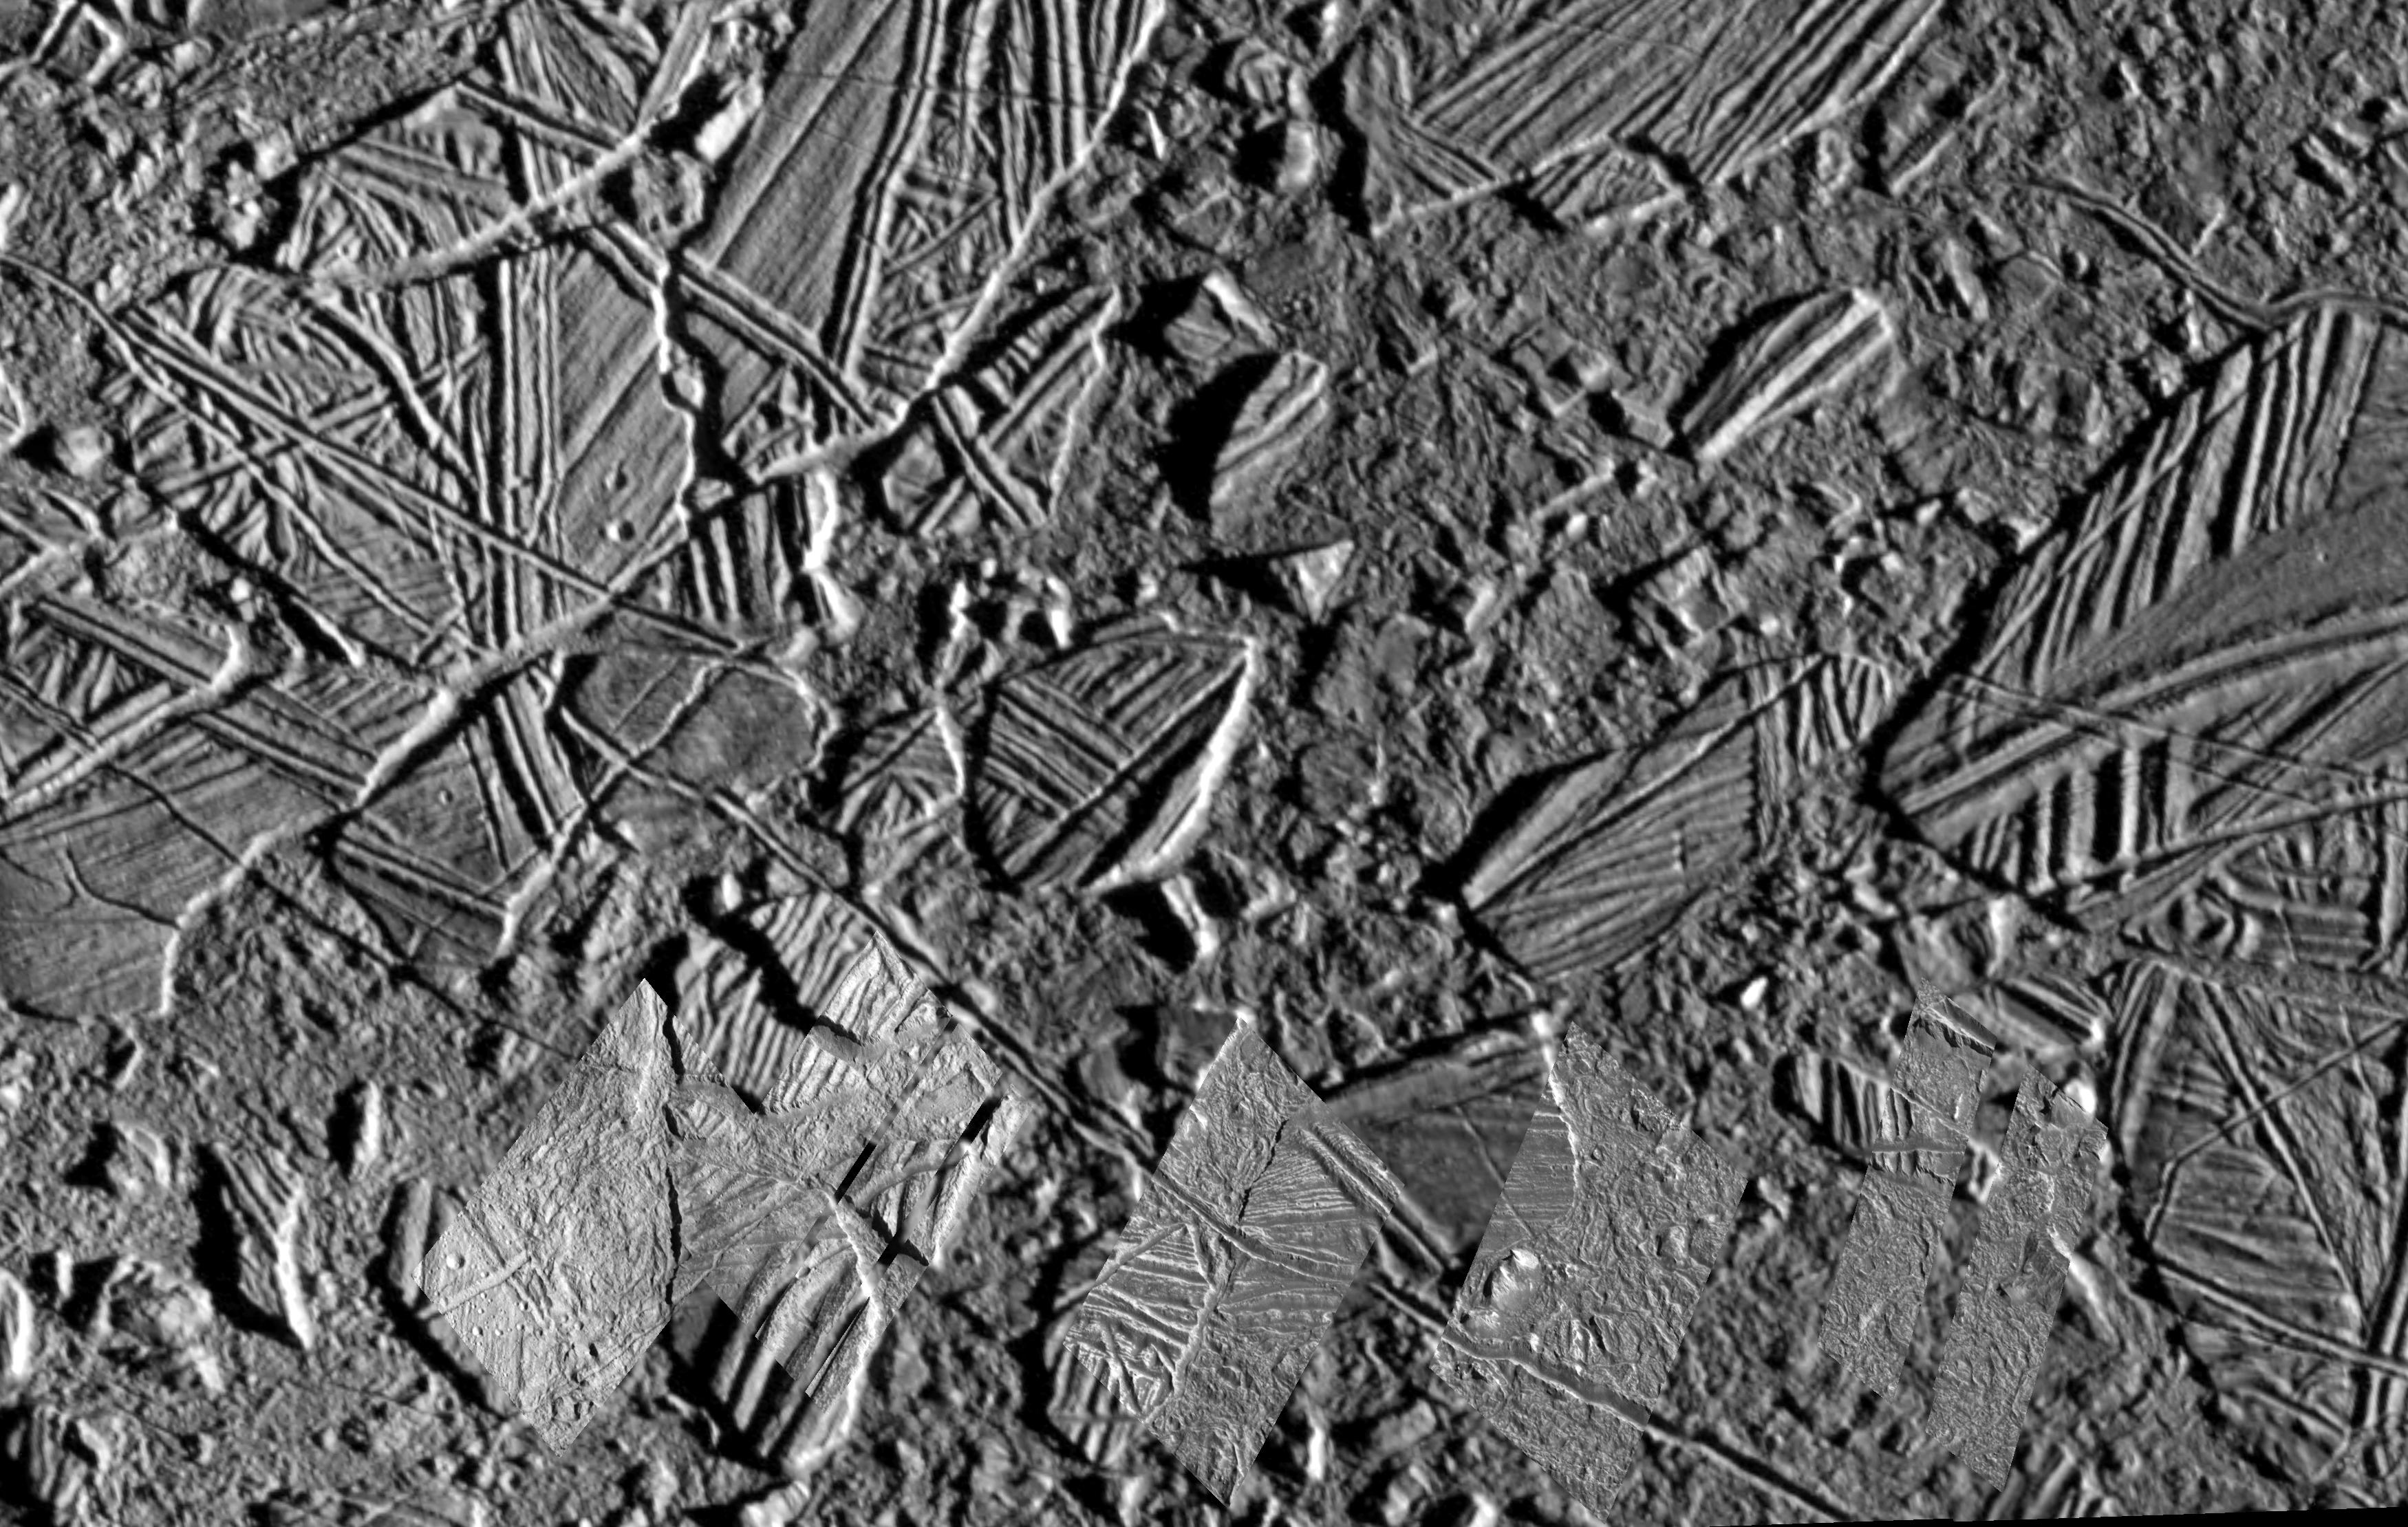
\includegraphics[width=.48\textwidth]{figures/edge/PIA01403}
	}
	\subfloat{
		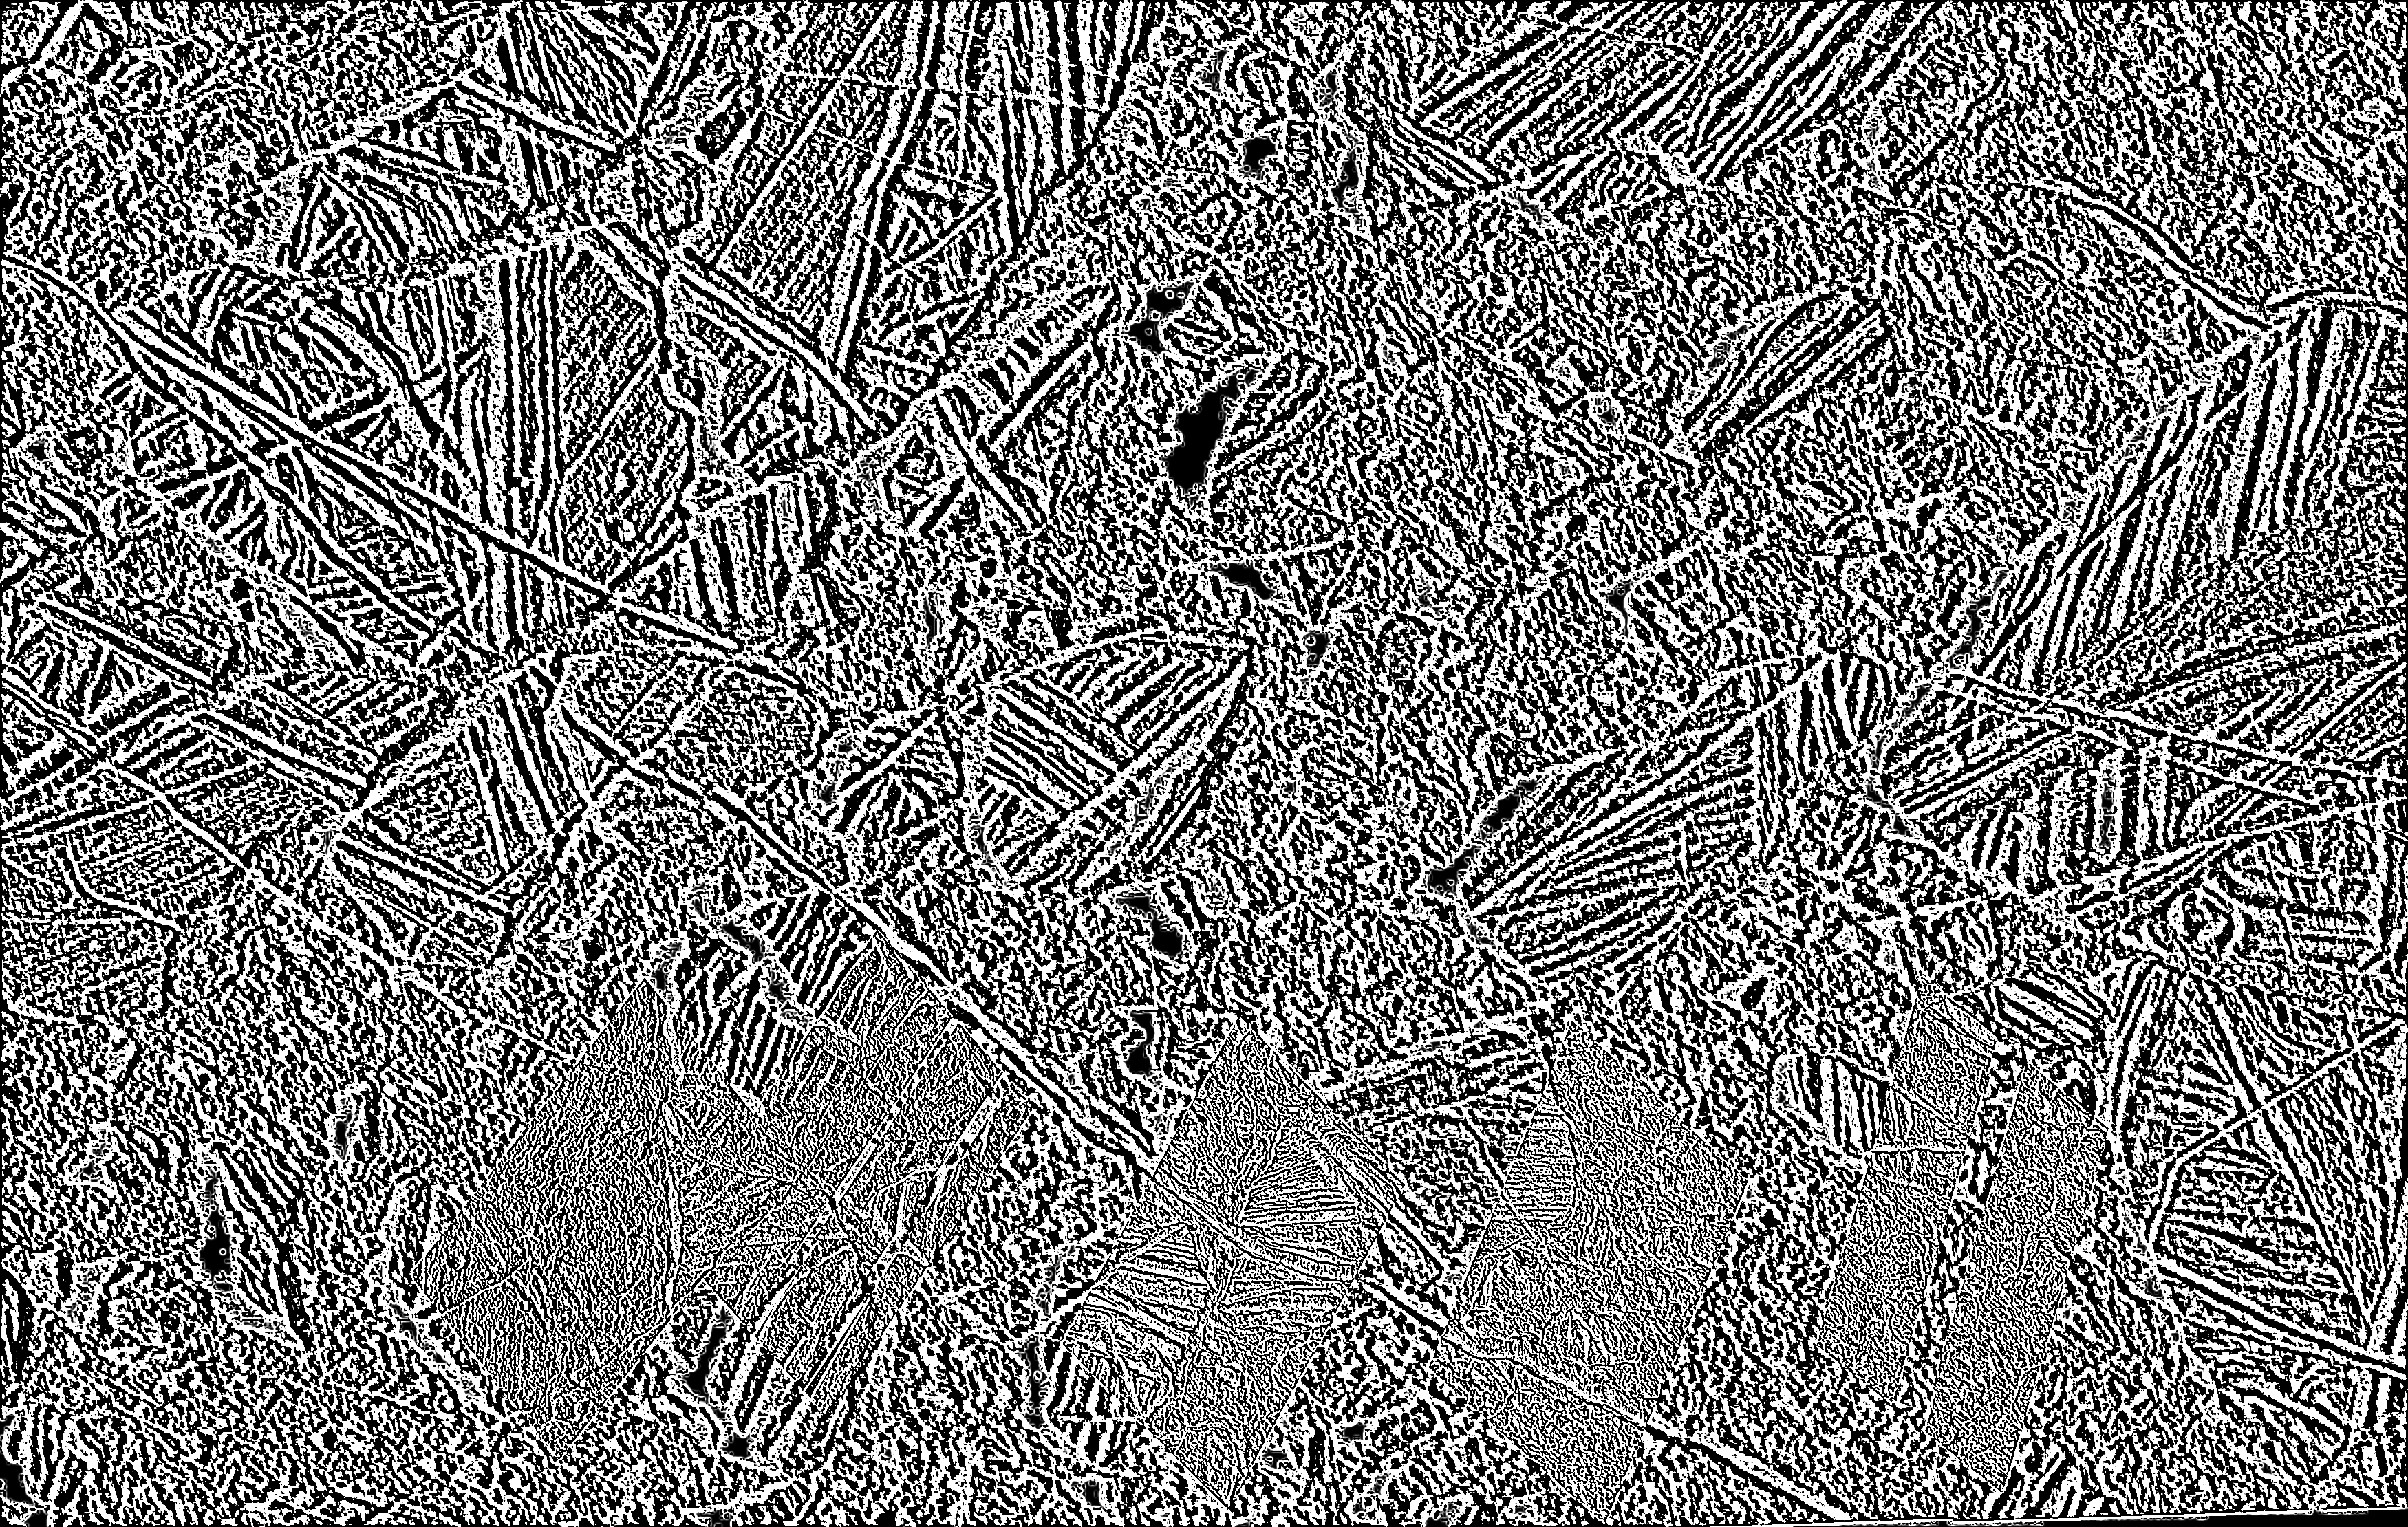
\includegraphics[width=.48\textwidth]{figures/edge/PIA01403_filtered}
	}
	\\
	\subfloat{
		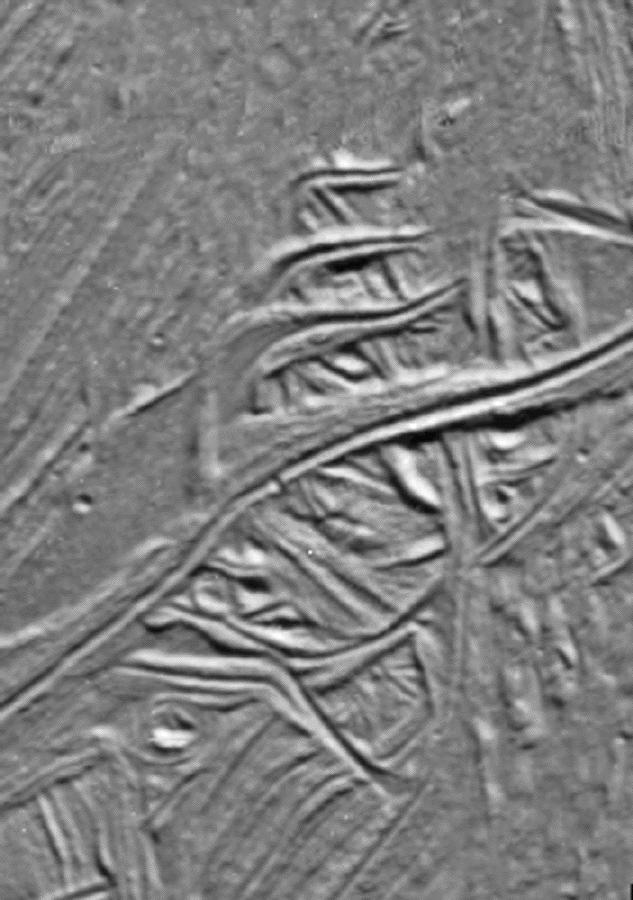
\includegraphics[width=.31\textwidth]{figures/edge/PIA01642}
	}
	\subfloat{
		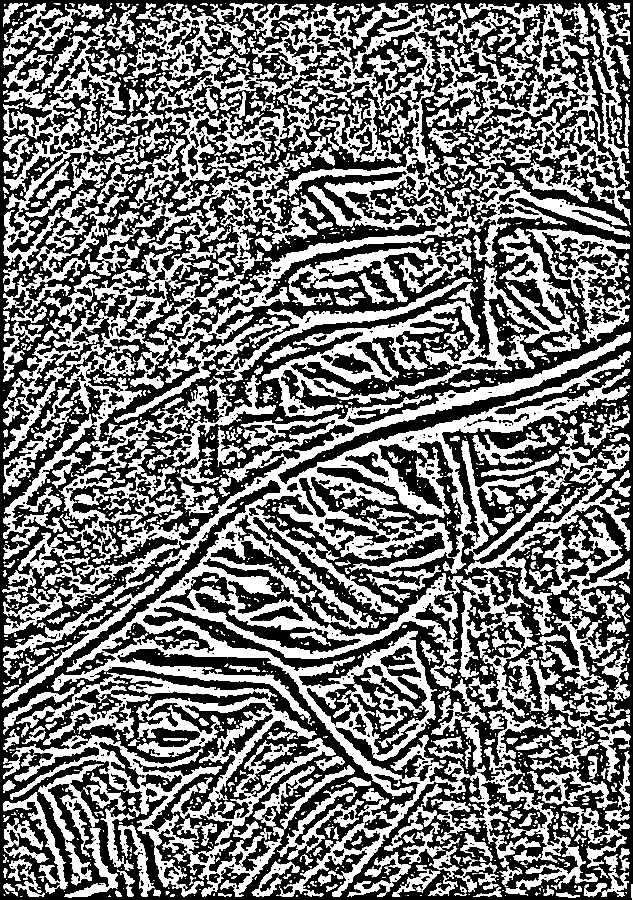
\includegraphics[width=.31\textwidth]{figures/edge/PIA01642_filtered}
	}
	\subfloat{
		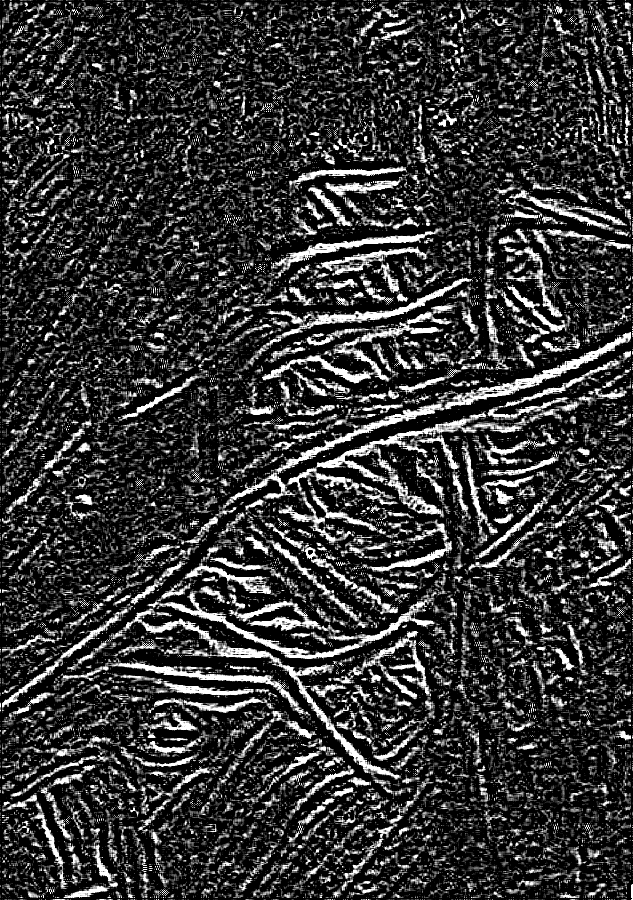
\includegraphics[width=.31\textwidth]{figures/edge/PIA01642_filtered_alternativ}
	}
	\captionsetup{width=.9\textwidth}
	\caption{Example of Laplacian Gaussian filter used for edge detection on the surface of the moon}
	\label{fig:edge_detection}
\end{figure}

\autsection{Radiation Shielding Theory}{Jean-Paul Breuer}
With regards to the instrumentation on board, there will need to be some type of shielding as protection against harmful radiation as well as from the potential heat generated by the RTG. Whenever gamma radiation passes through matter, it undergoes absorption via Compton, photoelectric, and pair-production interactions. Therefore, the intensity of the emitted radiation decreases as a function of thickness and density of the absorbing material, as stated by the Beer-Lambert law,
\begin{equation}
I = I_0 e^{-\alpha x}
\end{equation}

rearranging the relation and taking the log of both sides gives,\\
\begin{equation}
\ln\left( \frac{l_0}{l}\right) = \alpha x
\end{equation}

where then finding the half value layer (HVL), or where the initial intensity is halfed, can be computed through,\\
\begin{equation}
\ln(2) = \alpha x_{1/2} \Rightarrow x_{1/2} = \frac{0.693}{\alpha} \label{halfthickness}
\end{equation}
In other words, the more dense the material, the less thickness will be required to effectively attenuate the radiation. However, as mentioned previously, whenever radiation passes through matter, there are several interactions that can occur, including X-ray fluorescence.

The transition energy between two electron shells within an atom (typically higher shells K,L,M,+) is the same as the energy of characteristic radiation for that element, which manifests itself as the inner-shell ionization by an accelerated electron. Naturally, ionization can occur in several different electron levels, forming a characteristic spectrum for each element, since all transition energies are unique to each atom. This transition of an excited atom into a lower energy occurs via the photoelectric effect, where radiation ejects inner shell electrons, whereby electrons from the outer shells are transfered into the inner shells to fill in the vacancies, emitting a photon in the X-ray range that is unique to that element with energy equal to the transition energy $E_c = E_m - E_n$. This is the case for elements with higher atomic numbers; however, for elements with low atomic numbers, the Auger effect tends to dominate, where instead of the energy being emitted as a photon, it instead is transfered to another electron which is then ejected from the atom.

The empirical law for the characteristic X-ray emission from an atom is given by Moseley's Law,\\
\begin{equation}
E_c= R_h \cdot (Z-\sigma)^2 \left(\frac{1}{n^2} - \frac{1}{m^2}\right)\label{moseley:eq}
\end{equation}

where $R_h$ is the Rydberg constant, $Z$ is the atomic number, and $\sigma$ is the screening constant of the atom. It is then possible to estimate the energy of a $K_\alpha$ transition via the relation,\\
\begin{equation}
E_{K_\alpha} = A \cdot (Z-1)^2 \label{transition}
\end{equation}
where $A = 10.22$ eV is the $K_\alpha$ transition in hydrogen. Following Equation \ref{transition}, it is evident that every element has its own characteristic fingerprint, but more importantly, to create an effective shielding, it will be required to use several layers with different materials, to gradually attenuate all of the energy to a point where it will no longer damage the sensitive instrumentation. Given that the Orbiter will be orbiting Jupiter, with a heavy radiation environment, it will be very important to minimize the radiation as much as possible, especially during the Lander phase of the mission when the equipment will be most exposed to the harmful radiation from the planet.


%* Water, oil, fat, carbon, energy
%
%* Proteins (amino acids) etc
%
%* Nutritions, water, heat energy
%
%* How can a life-form be able to convert thermal energy to other forms of energy
%
%* Another energy source could be geysers on the solid core
%
%    * A probe to the ocean bottom might show this
%    
%* Lakes inside the ice
%
%* Iron-reduction
